\chapter{指数概念普遍化与对数}

\section{指数概念普遍化}
\subsection{引言}
这一节我们要把指数的概念加以推广,除了第一册学过
的整数指数、
零指数外,还要引入负整数指数,正、负分数
指数,为能够应用对数来简化乘法、除法、乘方、开方的计
算建立初步理论基础。

在推广过程中要注意以下几个方面:
\begin{enumerate}
\item 各种定义的条件。
\item 探索各种定义产生的逻辑过程,
\item 要熟练运用各种定义去计算。
\end{enumerate}


我们来回忆一下正整数指数幂的定义:

\begin{blk}{定义1}
$a^n=\overbrace{a\cdot a\cdots a}^{\text{$n$个}}$ ($n$是大于1的正整数),其中$a$称
为\textbf{底数},$n$称为\textbf{指数},$a^n$称为以$a$为底数、$n$为指数的\textbf{幂}.当$n=1$
时,规定$a^1=a$。
\end{blk}

在定义1中,对于底数$a$,没有任何限制,$a$
可以是正数,也可以是负数,也可以是零;而指数$n$,必须
是正整数,否则定义1就无意义!这样,我们称按定义1定
义的$a^n$为正整数指数幂。

我们可以证明正整数指数幂有下列性质:
\begin{blk}{性质}
\begin{enumerate}
    \item $a^m\cdot a^n=a^{m+n}$ \quad ($m,n$为正整数);
    \item $a^m\div a^n=a^{m-n}$\quad ($m,n$为正整数,且$m>n,\; a\ne 0$);
    \item $(a^m)^n=a^{mn}$\quad ($m,n$为正整数);
    \item $(ab)^n=a^nb^n$ \quad($n$为正整数);
    \item $\left(\frac{a}{b}\right)^n=\frac{a^n}{b^n}$\quad ($n$为正整数,$b\ne 0$)。
\end{enumerate}
\end{blk}

以后将会看到,将指数概念扩充到新的范围以后,这几
条性质依然保留,并且可以适当地合并。

\subsection{零指数与负整数指数}

【I】从正整数指数幂的性质可以看到:
\begin{itemize}
    \item 幂的\textbf{乘法}可以转化为指数\textbf{加法},(性质1)
    \item 幂的\textbf{除法}可以转化为指数\textbf{减法},(性质2)
    \item 幂的\textbf{乘方}可以转化指数\textbf{相乘}。(性质3)
\end{itemize}

要使正整数的加、减、乘、除,尤其是减、除通行无阻,
那么指数只限制在正整数范围是不行的,例如:$a^3\div a^2=
a^{3-2}=a^1=a$, 这个转化是没有问题的,但是
\[a^3\div a^3 \mathop{=}^{?} a^{3-3} \mathop{=}^{?} a^0=?\]
\[a^2\div a^4 \mathop{=}^{?} a^{2-4} \mathop{=}^{?} a^{-2}=?\]

要使指数的减法通行无阻,就会出现零指数和负整数指
数,而零指数和负整数指数是什么,过去从未见过,这就有
必要将指数的概念加以推广,给零指数和负整数下定义。

【II】探索零指数和负整数指数如何定义。

我们知道$a^m\div a^n=a^{m-n}$,
这里限制$a\ne 0$, 并且$m>n$, $m$、$n$均为正整数,现在把$m>
n$的条件取消,这样$m$可以等于$n$. 在$m=n$的时候,上面的公
式就是:
\[a^m\div a^n=a^n\div a^n=a^{n-n}=a^0\quad (a\ne 0)\]
而$a^m\div a^n$的实际内容是
\[a^m\div a^n=\frac{a^m}{a^n}=\frac{a^n}{a^n}=1\]

为了使公式$a^m\div a^n=a^{m-n}$
也适用于$m=n$的情况,就应该
使形式上的运算结果“$a^0$”与实际内容“1”一致起来,我们规
定$a$的零次幂等于1, 即$a^0=1\;\;  (a\ne 0)$就合理了。
用同样的方法,来探索$m<n$时的情况。

当$m<n$时,$a^m\div a^n=a^{m-n}=a^{-(n-m)}$,这里$-(n-m)$是个负整数,我们还没有规定$a^{-(n-m)}$的意
义。但另一方面,在$m<n$的条件下,$a^m\div a^n$的实际意义是:
\[a^m\div a^n=\frac{a^m}{a^n}=\frac{a^m\div a^n}{a^n\div a^n}=\frac{1}{a^{n-m}}\qquad (a\ne 0)\]
这样看来,为了使公式$a^m\div a^n=a^{m-n}$在$m<n$时也适用,规
定:
\[a^{-(n-m)}=\frac{1}{a^{n-m}}\quad (a\ne 0)  \]
就可以了,也就是说,$n$是正整数的时候,应规定:


【III】对零指数和负整数指数下定义

\begin{blk}{定义2}
    \[a^0=1\qquad  (a\ne 0)\]
\end{blk}

\begin{blk}{定义3}
    \[a^{-n}=\frac{1}{a^n} \qquad  (a\ne 0, \quad n\text{是正整数})\]
\end{blk}

这两个定义中特别要注意“$a\ne 0$”这个条件,也就是说零
的零次幂是没有意义的,零的负整数次幂也是没有意义的。

有了定义2和定义3, 对于同底数的整数指数幂相除的
运算法则,就可通行无阻,而不必再局限于$m>n$了,例
如
\[(-2)^2\div (-2)^2=(-2)^0=1\]
\[4^5\div 4^7=4^{5-7}=4^{-2}=\frac{1}{4^2}=\frac{1}{16}\]

定义1、2、3说明现在我们的指数已经扩充到整数范
围了。

【IV】性质的证明

一般来说,当一个概念被推广以后,原来具有的性质可
能有些仍然保持成立,有些就不再成立了。所以必须对原来
的性质逐条加以研究,对那些仍然成立的性质,加以证明肯
定,对那些不再成立的性质也应通过举反例加以否定。另
外,新的概念是否又带来了新的性质,这是研究推广了的概
念应该注意的一个问题,只有通过这样的研究,才能掌握推
广了的概念。

把指数概念推广到整数范围以后,上述五条性质,因条
件起了变化,就成为:

\begin{blk}{}
\begin{enumerate}
    \item $a^m\cdot a^n=a^{m+n}\quad (m,n\in\mathbb{Z},\;\; a\ne 0)$
    \item $a^m\div a^n=a^{m-n}\quad (m,n\in\mathbb{Z},\;\; a\ne 0)$
    \item $(a^m)^n=a^{mn}\quad (m,n\in\mathbb{Z},\;\; a\ne 0)$
    \item $(a\cdot b)^n=a^{n}\cdot b^n\quad (ab\ne 0,\;\; n\in\mathbb{Z})$
    \item $\left(\frac{a}{b}\right)^n=\frac{a^n}{b^n}\quad (ab\ne 0,\;\; n\in\mathbb{Z})$
\end{enumerate}    
\end{blk}

现在我们来证明性质1。

已知:$m,n$是任意两个整数,$a\ne 0$.

求证:$a^m\cdot a^n=a^{m+n}$

我们要对$m,n$分各种情况来讨论,由于$m,n$均可取正整
数、负整数和零,即
\[m=\begin{cases}
    0\\ \text{正整数}\\ \text{负整数}
\end{cases},\qquad n=\begin{cases}
    0\\ \text{正整数}\\ \text{负整数}
\end{cases}  \]
因而从$m$中取出一种情况,从$n$中取出一种情况,组成一种
情况,那么一共有$3\x3=9$种,在这九种情况中,因为$m
=$正整数,$n=$正整数的情况以前已证过,可以略去。又由
于实数乘法适合交换律,因而$m,n$是对称的,这样,我们只
就下面五种情况来证明:
\[\begin{cases}
    m=0\\n=0
\end{cases}\begin{cases}
    m=\text{正整数}\\n=0
\end{cases}\begin{cases}
    m=\text{负整数}\\n=0
\end{cases}\begin{cases}
m=\text{正整数}\\  n=\text{负整数}
\end{cases}\begin{cases}
    m=\text{负整数}\\  n=\text{负整数}
\end{cases}  \]

\textbf{情况1:} 当$m=0$, $n=0$时,由零指数的定义,
\[a^m\cdot a^n=a^0\cdot a^0=1\cdot 1=1=a^0=a^{m+n} \]
$\therefore\quad a^m\cdot a^n=a^{m+n}$成立。

\textbf{情况2:} 当$m$是正整数,$n=0$时,
\[a^m\cdot a^n=a^m\cdot a^0=a^m\cdot 1=a^m=a^{m+0}=a^{m+n}\]
$\therefore\quad a^m\cdot a^n=a^{m+n}$成立。


\textbf{情况3:} 当$m$是负整数,$n=0$时,
\[a^m\cdot a^n=a^m\cdot a^0=a^m\cdot 1=a^m=a^{m+0}=a^{m+n}\]
$\therefore\quad a^m\cdot a^n=a^{m+n}$成立。

\textbf{情况4:} 当$m$是正整数,$n$是负整数,那么$n=-|n|$, $|n|$为正整数。

$\because\quad a^m\cdot a^n=a^m\cdot a^{-|n|}=a^m\cdot\frac{1}{a^{|n|} }=\frac{a^m}{a^{|n|}}=a^{m-|n|}=a^{m+(-|n|)}=a^{m+n} $

$\therefore\quad a^m\cdot a^n=a^{m+n}$成立。

\textbf{情况5:} 当$m,n$都是负整数时,那么
$m=-|m|$, $n=-|n|$。因此:
\[\begin{split}
    a^m\cdot a^n&=a^{-|m|}\cdot a^{-|n|}=\frac{1}{a^{|m|}}\cdot \frac{1}{a^{|n|}}\\
    &=\frac{1}{a^{|m|}\cdot a^{|n|}}=\frac{1}{a^{|m|+|n|}}\\
    &=a^{-(|m|+|n|)}\\
    &=a^{-(|m|)+(-|n|)}=a^{m+n}
\end{split}\]
$\therefore\quad a^m\cdot a^n=a^{m+n}$成立。

综合五种情况及前面的分析,就证明了当$m,n$为任意整
数时,$a^m\cdot a^n=a^{m+n}$成立。

其它几条性质可以类似地证明。应当指出,有了定义2、3以后,对于任何整数$n$, 都有:
\[\frac{1}{a^n}=a^{-n}\qquad (a\ne 0)\]
这是因为:当$n$是正整数时,这就是定义3, 当$n$为零时,
 \[\frac{1}{a^n}=\frac{1}{a^0}=\frac{1}{1}=a^0=a^{-n}\]
 当$n$为负整数时,$n=-|n|$
\[\frac{1}{a^n}=\frac{1}{a^{-|n|}}=a^{|n|}=a^{-n}\]
这样,定义3虽然是对$n$为正整数来说的,有$a^{-n}=\frac{1}{a^n}$,
但实
际上暗示了$n$为任意整数时,$a^{-n}=\frac{1}{a^n}$
都有了确定的意义。

有了这个公式,上面的性质2就可归结到性质1
上。
事实上,只要1成立,那么对于任何整数$m,n$我们
有:
\[a^m\div a^n=a^m\cdot \frac{1}{a^n}=a^m\cdot a^{-n}=a^{m+(-n)}=a^{m-n}\]

有了这个公式,上面的性质5也可归结为性质3和4。
事实上,只要3和4成立,那么对于任何整数$m,n$,
我们有:
\[\begin{split}
    \left(\frac{a}{b}\right)^n&=\left(a\cdot\frac{1}{b}\right)^n=(a\cdot b^{-1})^n=a^n\cdot (b^{-1})^n\\
    &=a^n \cdot b^{-n}=a^n\cdot \frac{1}{b^n}=\frac{a^n}{b^n}
\end{split}\]
这样,五条性质可归结为三条性质:
\begin{enumerate}
    \item $a^m\cdot a^n=a^{m+n}\quad (a\ne 0;\;\;m,n\in\mathbb{Z})$
    \item $(a^m)^n=a^{mn}\quad (a\ne 0;\;\;m,n\in\mathbb{Z})$
    \item $(a\cdot b)^n=a^n\cdot b^n \quad (ab\ne 0;\;\;n\in\mathbb{Z})$
\end{enumerate}


\begin{example}
\begin{multicols}{2}  
    \begin{enumerate}
        \item $2^0=1$
        \item $(0.75)^0=1$
        \item $\left(-\sqrt{3}\right)^0=1$
        \item $0^0$无意义
        \item $10^{-3}=\frac{1}{10^3}=0.001$
        \item $3(-2)^{-4}=\frac{3}{(-2)^{4}}=\frac{3}{16}$
        \item $\left(\frac{1}{2}\right)^{-5}=2^5=32$
        \item $(-0.25)^{-1}=\left(-\frac{1}{4}\right)^{-1}=-4$
    \end{enumerate}
\end{multicols}   
\end{example}

\begin{example}
    把下列单项分式化成整式形式:
    \[\frac{a}{3bc^2}=\frac{1}{3}ab^{-1}c^{-2},\qquad \frac{3}{2a^{-3}b^{-1}c^2}=\frac{3}{2}a^3bc^{-2}  \]
\end{example}

\begin{example}
    把下面的数写成$a\cdot 10^n$的形式,这里$a$是含有一
位整数的数,$n$是任意整数(把一个数写成这种形式叫 科学
记数法)。
    \begin{enumerate}
        \item 1吨(t)$=1000$公斤(kg)$=10^3$公斤(kg)
        \item  1毫米(mm)$=0.001$米(m)$=10^{-3}$米(m)
        \item  1年$=31,556,925,975$秒(s)=$3.1556925975\x10^7$(s)$\approx 3.156\x10^7$(s)
        \item   地球到太阳的距离$=149,640,000$公里(km)
        $=1.4964\x10^8$(km)
        \item    地球的质量$=5,970,000,000,000,000,000,000$(t)
        $=5.97\x10^{21}$(t)
        \item    原子核$U_{288}$的半径$=0.000,000,000,000,93$(cm)$=9.3\x10^{-13}$(cm)
    \end{enumerate}
\end{example}

\begin{example}
\begin{enumerate}
    \item $(b^{-3})^{-2}=b^{(-3)(-2)}=b^6$
    \item \[\begin{split}
        \left(3a^{-2}b^2c^{-3}\right)\left(\frac{4}{5}ab^{-3}c^3\right)&=\frac{12}{5}a^{-2+ 1}b^{2+(-3)}c^{-3+3}\\
        &=\frac{12}{5}a^{-1}b^{-1}\\
        &=\frac{12}{5ab}
    \end{split}\]
    \item \[\begin{split}
        \left(\frac{a+b}{a-b}\right)^{-3}\left(\frac{a-b}{a+b}\right)^{-2}&=\left[\left(\frac{a+b}{a-b}\right)^{-1}\right]^{3} \left(\frac{a-b}{a+b}\right)^{-2}\\
        &=\left(\frac{a-b}{a+b}\right)^{3}\left(\frac{a-b}{a+b}\right)^{-2}\\
        &=\left(\frac{a-b}{a+b}\right)^{3-2}=\left(\frac{a-b}{a+b}\right)^{1}\\
        &=\frac{a-b}{a+b}
    \end{split}\]
\end{enumerate}
\end{example}

    
\begin{example}
\begin{enumerate}
    \item \[\begin{split}
        \frac{\left(a^{-2} b^{-3}\right)\left(-4 a^{-1} b\right)}{12 a^{-4} b^{-2}}&=\frac{-4 a^{-2-1} b^{-3+1}}{12 a^{-4} b^{-2}} \\
    &=\frac{-4 a^{-3} b^{-2}}{12 a^{-4} b^{-2}}\\
    &=-\frac{1}{3} a
    \end{split}\]
    \item \[\begin{split}
        \left(x^{2}-y^{-2}\right)\div\left(x-y^{-1}\right) 
    &=\left[x^{2}-\left(y^{-1}\right)^{2}\right] \div\left(x-y^{-1}\right) \\
    &=\left(x+y^{-1}\right)\left(x-y^{-1}\right)\div \left(x-y^{-1}\right) \\
    &=x+y^{-1}=x+\frac{1}{y}
    \end{split}\]
\end{enumerate}
\end{example}


\section*{习题1.1}
\addcontentsline{toc}{subsection}{习题1.1}

\begin{enumerate}
    \item 换去下列各算式中的负指数:
    \begin{multicols}{2}
        \begin{enumerate}
        \item $4x^{-3}y^3$
        \item $\frac{1}{5c^{-3}}$
        \item $\frac{4a^{-2}}{5b^{-3}}$
        \item $\frac{3a^{-3}x^2}{5b^3y^{-4}}$
    \end{enumerate}
    \end{multicols}
    
    \item 证明下面的运算法则,如果$m,n$为任意整数,而$a\ne 0$,
    则$(a^m)^n=a^{m\cdot n}$
    \item 把下列的数写成$a\cdot 10^n$的形式,这里$a$是含有一位整数的数,$n$是任意整数,
    \begin{multicols}{2}
        \begin{enumerate}
        \item 8900
        \item  3,200,000
        \item 0.000,015
        \item 0.000,000,025
    \end{enumerate}
    \end{multicols}
    
    
\item 下面是物理学常用的长度单位,将它化成mm并以10的幂表
示出来:
\begin{enumerate}
    \item $1\text{微米}(1\mu {\rm m})=\frac{1}{1000}{\rm mm}$
    \item $1\text{毫微米}(1 {\rm nm})=\frac{1}{1,000,000}{\rm mm}$ 
    \item  $1\text{微微米}(1 {\rm pm})=\frac{1}{1,000,000,000}{\rm mm}$ 
\end{enumerate}


\item 以10的幂来表示:
\begin{enumerate}
    \item 1mm是多少cm;
    \item 1${\rm cm}^3$是多少${\rm m}^3$ (Litre即升);
    \item 1g是多少kg, 是多少吨(t)。
\end{enumerate}
\item 将下面的数据用小数形式表示出来:
\begin{enumerate}
    \item 红血球的直径$=0.7\x10^{-8}$(cm);
    \item 最小的细菌的长度$\approx 10^{-4}$(cm);
    \item 钠光(黄色)的波长$=5.89\x10^{-7}$(cm);
    \item 氢原子的直径$\approx 10^{-8}$(cm);
    \item 氢原子的质量$=1.64\x10^{-24}$(g);
    \item 电子的质量$=9\x10^{-28}$(g);
    \item 铀矿石的含镭量$=3.328\x10^{-6}$\%.
\end{enumerate}

\item 完成下列运算并将所得结果中的负指数变换成正指数:
\begin{multicols}{2}
 \begin{enumerate}
    \item $(2x^2)\div (3x^{-3})$
    \item $ax^2\div x^{-1}$
    \item $(a^{-2}x^2)\div a^4$
    \item $(ax)^{-3}\div (bx)^{-3}$
    \item $(2^n)^{n-1} \div (2^{n-1})^{n+1}\quad (n>1)$
\end{enumerate}   
\end{multicols}

\item 利用整数指数幂的指数法则,计算
\begin{multicols}{2}\begin{enumerate}  
\item $\left\{\left[\frac{5}{3}-\left(\frac{6}{5}\right)^{-1}\right]^{-2}-\left(\frac{25}{11}\right)^{-1}\right\}^{-3}$\item $\left[\left(\frac{5 a^{-2} c^{3}}{3 x^{-3} y^{4}}\right)^{-2}\right]^{4}$
\item $\frac{\left(3 x^{2} y^{-3}\right)^4}{\left(-2 x^{-3} y^{2}\right)^{-3}\left(-27 x^{-5} y^{2}\right)}$
\item $\left(\frac{2}{a^{n}+a^{-n}}\right)^{-2}-\left(\frac{2}{a^{n}-a^{-n}}\right)^{-2}$
\end{enumerate}\end{multicols}

\item 求证:
\begin{enumerate}
    \item $\left(a+a^{-1}\right)^{2}\left(a-a^{-1}\right)^{2}=a^{4}-2+\frac{1}{a^{4}}$
    \item $\frac{a^{-3}+b^{-3}}{a^{-1}+b^{-1}}+\frac{a^{-3}-b^{-3}}{a^{-1}-b^{-1}}=2\left(\frac{1}{a^{2}}+\frac{1}{b^{2}}\right)$
\end{enumerate}

\item 化简:
 \begin{multicols}{2}
\begin{enumerate}
    \item  $\frac{a^{2}+a^{-2}-2}{a^{2}-a^{-2}}$
    \item  $\frac{m^{3}+n^{-3}}{m+n^{-1}}+\left(m-n^{-1}\right)^{2}$
\end{enumerate}
\end{multicols}
\item 求$32x^{-6}+12x^{-4}+10x^{-2}-12$除
以$2x^{-2}-1$所得的商式
和余数。
\end{enumerate}

\subsection{$n$次算术根}
为了进一步把指数概念从整数范围扩充到有理数范围,
我们先介绍一下$n$次算术根及其运算性质。

\begin{blk}{定义}
 设$a$是一个实数,$n$是正整数,如果存在着实数
$x$, 使得
$$x^n=a$$
那么,$x$就叫做\textbf{$a$的$n$次方根},$a$叫做\textbf{被开方数},$n$叫做\textbf{根指数}。   
\end{blk}
 
由方根的定义推知:
\begin{enumerate}
    \item 如果$x_1$是正数$a$的偶次方根,那么$x_1$也是$a$的偶次
    方根。

    因为如果存在$x_1$使得$x_1^n=a\; (>0)$, 那么,$(-x_1)^n=(x_1)^n=a$ ($n$为偶数),即$x_1$和$-x_1$都是正数$a$的偶次方根.比如,
$x^4=16$, 则$x=\pm 2$都是16的四次方根。
\item 负数的偶次方根不存在,这是因为任何数的偶次方
都是非负数的缘故。
\item 不等于零的任何数的奇次方根的符号与被开方数的
符号相同。

因为如果被开方数是负数$-a\; (a>0)$, 那么它的奇次方
根,就不能是0或正数,由于0的任何奇次方是0, 正数的
任何奇次方是正数,这就说明负数的奇次方根应该是负数;
同样说明正数的奇次方根应该是正数。
\item 0的方根是0。
\end{enumerate}

在本教程的第六册中,我们将证明下面的存在定理。


\begin{blk}{定理}
    如果$a>0$, 方程$x^n=a$存在唯一的正实数根。
\end{blk}

为明确起见,我们把这个正实数方根叫做$a$的算术根,下
面给出它的定义和记法。


\begin{blk}{定义}
    如果$a$是正实数,那么$a$的正的$n$次方根叫做\textbf{$a$的$n$次
算术根},而零也叫零的$n$次算术根,记为$\sqrt[n]{a}$。$a$的算术平方根
用不带根指数的符号$\sqrt{n}$表示。$\sqrt[1]{a}$这个表示$a$的符号,我们不用。
\end{blk}

例如:$2^6=32$, 2叫做32的5次方根,也是32的5次算术根,
因此$\sqrt[5]{32}=2$; $(\pm 2)^4=16$,$2$和$(-2)$都是16的4次方根,其中2是16的4次算术根,因此$\sqrt[4]{16}=2$; $(-2)$不是16的4次算术根。因此$\sqrt[4]{16}\ne -2$, 但$-2$可写成$-\sqrt[4]{16}$。$(-3)^3=-27$, $-3$
叫做$-27$的3次方根,但不是算术根。有的课本也用符号$\sqrt[n]{a}$
($a<0$, $n$是奇数)表示负数的奇次方根,例如$\sqrt[3]{-27}=-3$。
但是负数的奇次方根总可以用对应的算术根表示出来,例如
$\sqrt[3]{-27}=-\sqrt[3]{27}$, 一般地,$\sqrt[2n+1]{-a}=-\sqrt[2n+1]{a}\quad  (a>0)$。

请注意以下几点:

\begin{enumerate}
    \item 算术根的概念含有两个条件:被开方数是非负的;
算术根只代表方根中的非负值。以后在实数范围内,符号
$\sqrt[n]{a}$($a>0$)只代表算术根,因此,正数$a$的偶次方根的负值
用$-\sqrt[n]{a}$表示。
\item 在等式$x^n=a$中,已知$x$和$n$求$a$的过程叫做乘方运算。
反过来,已知$a$和$n$求$x$的过程叫做开方运算,乘方运算和开
方运算互为逆运算,由于当$a\ge 0$时,$\sqrt[n]{a}$是非负值,因此对
于一切大于1的正整数$n$都有:
\begin{align}
    \left(\sqrt[n]{a}\right)^n&=a\\
    \sqrt[n]{a^n}&=a
\end{align}

事实上,设$\sqrt[n]{a}=x$, 按定义,$x^n=a$, 所以$\left(\sqrt[n]{a}\right)^n=a$。

在$a<0$的场合,可以验知:当$n$是奇数时,等式(1.1)、
(1.2)对于负数的奇次方根仍保持;而当$n$是偶数时,等式(1.1)
无意义,而(1.2)的右端是$|a|$, 不是$a$, 即$a=|a|$, 这是因
为算术根只代表非负数的缘故。

例如:$\sqrt{(-2)^2}+\sqrt[3]{-27}+\sqrt[5]{243}=\sqrt{(-2)^2}+\sqrt[3]{(-3)^3}+\sqrt[5]{3^5}=2-3+3=2$

\item 符号$\sqrt[n]{\quad }$叫做$n$次根号,如果根号下是一个算式,例如$\sqrt{1-a}$,$\sqrt[3]{\frac{x}{y}}$
等等,我们称它为根式。当根号下的算式
的值不为负数时,它的$n$次算术根才有意义。

例如:$\sqrt{(a-2)^2}=\begin{cases}
    a-2 & a\ge 2\\
    2-a & a<2
\end{cases},\quad \sqrt{(1-a)} \text{ 在$a\le 1$的情形下有意义}$

\end{enumerate}

下面我们介绍$n$次算术根的性质。

\begin{blk}{性质1:乘积的开方法则}
设$n$为正整数,$a,b$为正实数,那么
$$\sqrt[n]{ab}=\sqrt[n]{a}\cdot \sqrt[n]{b}$$
\end{blk}

\begin{proof}
    因为$\left(\sqrt[n]{a}\cdot \sqrt[n]{b}\right)^n=\left(\sqrt[n]{a}\right)^n\cdot \left(\sqrt[n]{b}\right)^n=ab$
    
    按方根定义,$\sqrt[n]{a}\cdot \sqrt[n]{b}$是$ab$的$n$次方根,又因为$a,b$是正
    数,当然积$ab$仍是正数,且算术根的积$\sqrt[n]{a}\cdot \sqrt[n]{b}$也是正数,
    这就是说,$\sqrt[n]{a}\cdot \sqrt[n]{b}$是正数$ab$的$n$次算术根;另一方面,$ab$
    的$n$次算术根是$\sqrt[n]{ab}$, 根据$ab$的$n$次算术根的唯一性得到
    $$\sqrt[n]{ab}=\sqrt[n]{a}\cdot \sqrt[n]{b}$$
\end{proof}

\begin{blk}{推论}
\[\sqrt[n]{a_1a_2\cdots a_n}=\sqrt[n]{a_1}\cdot \sqrt[n]{a_2}\cdots \sqrt[n]{a_n}\]
\end{blk}

例如:\[\begin{split}
    \sqrt[3]{60\x 18\x 25}&=\sqrt[3]{(2^2\x 3\x 5)(2\x 3^2)(5^2)}\\
    &=\sqrt[3]{2^3\x 3^3\x 5^3}\\
    &=2\x 3\x 5=30
\end{split}\]

\begin{blk}{性质2:幂的开方法则}
设$m,n$是正整数,$a>0$, 那么,$\sqrt[n]{a^m}=\left(\sqrt[n]{a}\right)^m$。

\end{blk}

\begin{proof}
由性质1的推论得,
\[\sqrt[n]{a^m}=\underbrace{\sqrt[n]{a\cdot a\cdots a}}_{\text{$m$个}}=\underbrace{\sqrt[n]{a}\cdots \sqrt[n]{a}}_{\text{$m$个}}=\left(\sqrt[n]{a}\right)^m\]
\end{proof}

\begin{blk}{性质3:商的开方法则}
    设$n$为正整数,$a,b>0$, 那么,
\[\sqrt[n]{\frac{a}{b}}=\frac{\sqrt[n]{a}}{\sqrt[n]{b}}\] 
\end{blk}

\begin{proof}
$\because\quad \left(\frac{\sqrt[n]{a}}{\sqrt[n]{b}}\right)^n=\frac{\left(\sqrt[n]{a}\right)^n}{\left(\sqrt[n]{b}\right)^n}=\frac{a}{b}$

又$\because\quad a>0,\quad   b>0,\quad \frac{a}{b}>0,\quad \frac{\sqrt[n]{a}}{\sqrt[n]{b}}>0$

$\therefore\quad \frac{\sqrt[n]{a}}{\sqrt[n]{b}}$是$\frac{a}{b}$的$n$次算术根

$\therefore\quad \sqrt[n]{\frac{a}{b}}=\frac{\sqrt[n]{a}}{\sqrt[n]{b}}$

\end{proof}

\begin{blk}{性质4:根式的开方法则}
    设$m,n$是正整数,$a>0$, 那么,
\[\sqrt[m]{\sqrt[n]{a}}=\sqrt[mn]{a}\]
\end{blk}

\begin{proof}
    $\because\quad \left(\sqrt[m]{\sqrt[n]{a}}\right)^{mn}=\left[\left(\sqrt[m]{\sqrt[n]{a}}\right)^m\right]^n=\left(\sqrt[n]{a}\right)^n=a$

    又$\because\quad a>0,\quad \sqrt[m]{\sqrt[n]{a}}>0 $
    
    $\therefore\quad \sqrt[n]{a}$是$a$的$mn$次算术根,

    $\therefore\quad \sqrt[m]{\sqrt[n]{a}}=\sqrt[mn]{a}$
\end{proof}


\begin{blk}{性质5:幂指数与根指数相约法则}
设$m,n,k$为正整数,$a>0$, 那么,
\[\sqrt[nk]{a^{mk}}=\sqrt[n]{a^m} \]  
\end{blk}

\begin{proof}
$\because\quad \left(\sqrt[n]{a^m}\right)^{nk}=\left[\left(\sqrt[n]{a^m}\right)^n\right]^k=\left(a^m\right)^k=a^{mk}$

又$\because\quad a>0,\quad \sqrt[n]{a^m}>0,\quad a^{mk}>0 $
    
$\therefore\quad \sqrt[n]{a^m}$是$a^{mk}$的$nk$次算术根,

$\therefore\quad \sqrt[nk]{a^{mk}}=\sqrt[n]{a^m} $
\end{proof}

最后强调,这些性质是在$a>0$的前提下成立的,对于
$a<0$, 有些根式也许仍有意义,但法则就不适用了,例如,性
质5:

设$a=-8$, 那么,
$\sqrt[6]{(-8)^2}=\sqrt[6]{64}=2$, 而$\sqrt[3]{-8}=\sqrt[3]{(-2)^3}=-2$,
因此,$\sqrt[6]{(-8)^2}\ne \sqrt[3]{-8}$。



\begin{example}
    化简下列各式:
\begin{enumerate}
\item $\sqrt[4]{25 x^{2} y^{2}} \quad(x, y \ge 0)$
\item  $\sqrt[6]{5^{4} a^{4} b^{2}}\quad (a, b \ge 0)$
\item $\sqrt{3 x^{2 a+2}}\quad (x \ge 0)$
\item $\sqrt[6]{27(u+v)^{18}}\quad (u,v\ge 0)$
\item $(a-b) \sqrt{\frac{a^{2}+a b}{a^{2}-2 a b+b^{2}}}\quad (a, b>0)$
\item $\sqrt[3]{16 \sqrt{2}}$
\item $\sqrt[4]{4 x^{6}}\quad (x \in \mathbb{R})$
\end{enumerate}
\end{example}

\begin{solution}
\begin{enumerate}
    \item $\sqrt[4]{25 x^{2} y^{4}}=\sqrt[4]{\left(5 x y^{2}\right)^{2}}=\sqrt{5 x y^{2}}$
    \item $\sqrt[6]{5^{4} a^{4} b^{2}}=\sqrt[6]{\left(5^{2} a^{2} b\right)^{2}}=\sqrt[3]{5^{2} a^{2} b}=\sqrt[3]{25 a^{2} b}$
    \item $\sqrt{3 x^{2 n+2}}=\sqrt{3} \cdot \sqrt{\left(x^{n+1}\right)^{2}}=\sqrt{3} x^{n+1}$
    \item \[\begin{split}
        \sqrt[6]{27(u+v)^{18}}&=\sqrt[6]{3^3\left[(u+v)^{6}\right]^{3}}\\
        &=\sqrt[6]{[3 (u+v)^{6}]^3}=\sqrt{3(u+v)^{6}}
        \\
        &=\sqrt{3}\sqrt{(u+v)^6}=\sqrt{3}(u+v)^3
    \end{split}\]
    \item \[\begin{split}
        (a-b) \sqrt{\frac{a^{2}+a b}{a^{2}-2 a b+b^{2}}}&=(a-b) \frac{\sqrt{a^2+ab}}{\sqrt{(a-b)^2}}\\
        &=(a-b)\frac{\sqrt{a(a+b)}}{|a-b|}\\
        &=\begin{cases}
            \sqrt{a(a+b)}, & a>b>0\\
            -\sqrt{a(a+b)}, & b>a>0
        \end{cases}
    \end{split}\]
\item \[\begin{split}
    \sqrt[3]{16 \sqrt{2}}&=\sqrt[3]{\sqrt{16^2}\cdot \sqrt{2}}\\
    &=\sqrt[3]{\sqrt{16^2 \cdot 2}}=\sqrt[6]{16^2 \cdot 2}\\
    &=\sqrt[6]{2^8\cdot 2}=\sqrt[6]{2^9}=\sqrt{2^3}=2\sqrt{2}
\end{split}\]
\item \[\begin{split}
    \sqrt[4]{4 x^{6}}&=\sqrt[4]{2^2 |x|^{6}}=\sqrt{2|x|^3}\\
    &=\sqrt{2\cdot |x|^2\cdot |x|}=\sqrt{2}|x|\sqrt{|x|}\\
    &=\begin{cases}
        \sqrt{2}x\sqrt{x} , & x\ge 0\\
        -\sqrt{2}x\sqrt{-x} , & x<0
    \end{cases}
\end{split}\]
\end{enumerate}
\end{solution}


\begin{example}
    把$\sqrt{2}$,$\sqrt[3]{-3}$,$\sqrt[4]{4}$化成同次式(指数相同的
    根式叫做同次根式)
\end{example}

\begin{solution}
$\because\quad \sqrt[3]{-3}=-\sqrt[3]{3},\quad \sqrt[4]{4}=\sqrt{2}$

$\therefore\quad $只需要考虑将$\sqrt{2}$, $\sqrt[3]{3}$化成同次根式
\[\begin{split}
\sqrt{2}&=\sqrt[6]{2^3}=\sqrt[6]{8}\\
\sqrt[3]{-3}&=-\sqrt[3]{3}=-\sqrt[6]{3^2}=-\sqrt[6]{9}\\
\sqrt[4]{4}&=\sqrt{2}=\sqrt[6]{8}
\end{split}\]
\end{solution}

\begin{ex}
\begin{enumerate}
    \item 求出下列方根的值:
    \begin{multicols}{2}
\begin{enumerate}
    \item $\sqrt[4]{10000}$
    \item $\sqrt[4]{1}$
    \item $\sqrt[4]{256}$
    \item $\sqrt[4]{\frac{1}{16}}$
    \item $\sqrt[4]{\frac{1}{625}}$
    \item $\sqrt[5]{100000}$
    \item $\sqrt[5]{0}$
    \item $\sqrt[5]{0.00001}$
    \item $\sqrt{\frac{4}{9}}$
    \item $\sqrt[4]{\frac{1}{81}}$
    \item $\sqrt[6]{64}$
    \item $\sqrt[3]{0.064}$
    \item $\sqrt[5]{0.00243}$
    \item $\sqrt[10]{0}$
    \item $\sqrt[3]{-2 \frac{10}{27}}$
\end{enumerate}        
    \end{multicols}

\item 计算下面方根,准确到0.1
\[\sqrt[4]{25},\qquad \sqrt[6]{27},\qquad \sqrt[8]{16},\qquad \sqrt[10]{32} \]

\item 约简下列根式中被开方数的指数和根指数:
\begin{multicols}{2}
\begin{enumerate}
    \item $\sqrt[6]{36 x^{2}}$
    \item $\sqrt[4]{25 y^{2}}$
    \item $\sqrt[8]{2^{4} a^{4} b^{6}}$
    \item $\sqrt[16]{14^{4^{4m} b^{8m}}}$
\end{enumerate}
\end{multicols}
这里,$a>0,\;\; b>0,\quad x,y\in\mathbb{R}$


\item 计算下列各题(题中字母都是正的):
\begin{multicols}{2}
    \begin{enumerate}
    \item $\sqrt[3]{\frac{8 x^{3} y^{6}}{27 x^{6} y^{9}}}$
    \item $\sqrt[n]{\frac{a^{n} b^{2n}}{x^{3 n} y^{n}}}$
    \item $\sqrt{\frac{25(a+b)^{2}}{(c-d)^{4}}}$
    \item $\sqrt[3]{-\frac{(a-b)^{3 n}}{(x+y)^{6n}}}$
    \item $\sqrt[n]{\frac{(a+b)^{2 n}}{a^{3 n}(a-b)^{n}}}$
\end{enumerate}
\end{multicols}

\item 化简下列各式:
\begin{multicols}{2}
    \begin{enumerate}
    \item $\sqrt{2 \sqrt{3}}$
    \item $\sqrt[3]{2 \sqrt{5}}$
    \item $\sqrt{3\sqrt[3]{2}}$
    \item $\sqrt[4]{5 \sqrt{2}}$
    \item $\sqrt{\sqrt[3]{a^{4} b^{2}}}$
    \item $\sqrt{x^{3} \sqrt[3]{x}}$
    \item $\sqrt{\frac{x}{y} \sqrt{\frac{x}{y}}}$
    \end{enumerate}
\end{multicols}
\end{enumerate}
     
\end{ex}


\subsection{最简根式和同类根式}
根式作运算,计算结果用根式表示时,根式应为最简根
式,最简根式指:
\begin{enumerate}
    \item 被开方数的每一个因式的指数都小于根指数;
    \item 根号内的式子不含分母;
    \item 根指数与被开方
数的指数互质。
\end{enumerate}

把根式化为最简根式的方法是:
\begin{enumerate}
    \item 移因式到根号外,例如:\[\sqrt[n]{a^nb}=\sqrt[n]{a^n}\cdot \sqrt[n]{b}=a\sqrt[n]{b}\;\;(a\ge 0)\]
    \item 移因式到根号内,例如:\[a\sqrt[3]{\frac{1}{a^2}}=\sqrt[3]{a^3}\cdot \sqrt[3]{\frac{1}{a^2}}=\sqrt[3]{\frac{a^3}{a^2}}=\sqrt[3]{a}\;\;(a>0)\]
    \item 化去根号内式子的分母,例如
    \begin{enumerate}
        \item 如果$ab>0$, 那么$\sqrt{\frac{a}{b}}=\sqrt{\frac{ab}{b^2}}=\frac{\sqrt{ab}}{\sqrt{b^2}}=\frac{\sqrt{ab}}{|b|}$
        \item 如果$a>0$, $b>0$, 且$n>m$, 那么
        \[\sqrt[n]{\frac{a}{b^m}}=\sqrt[n]{\frac{ab^{n-m}}{b^mb^{n-m}}}=\frac{\sqrt[n]{ab^{n-m}}}{\sqrt[n]{b^n}}=\frac{\sqrt[n]{ab^{n-m}}}{b} \]
    \end{enumerate}
\item 约去根指数与被开方数的指数的公因数,例如,
\[\sqrt[6]{8x^3}=\sqrt[6]{(2x)^3}=\sqrt{2x}\quad (x>0)\]
\end{enumerate}

\begin{example}
    化下面根式为最简根式:
\begin{enumerate}
    \item \[\begin{split}
        \frac{5 a^{2}}{7 b}\sqrt{\frac{49 b^{3}}{5 a}} &=\frac{5 a^{2}}{7 b} \sqrt{\frac{\left(7^{2} b^{2} b\right)(5 a)}{5^{2} a^{2}}} \\
    &=\frac{5 a^{2}}{7 b} \cdot \frac{7 b}{5 a} \sqrt{5 a b} \\
    &=a \sqrt{5 a b} \qquad(a>0, b>0) \\
    \end{split}\]
    \item \[\begin{split}
        \frac{2 a^{2}}{3 b} \sqrt[3]{\frac{b^{3}}{a^{4}}-\frac{b^{5}}{a^{6}}} &=\frac{2 a^{2}}{3 b}\sqrt[3]{\frac{a^{2} b^{3}-b^{5}}{a^{6}}} \\
    &=\frac{2 a^{2}}{3 b} \sqrt[3]{\frac{b^{3}\left(a^{2}-b^{2}\right)}{a^{6}}} \\
    &=\frac{2 a^{2}}{3 b} \cdot \frac{b}{a^{2}} \cdot \sqrt[3]{a^{2}-b^{2}} \\
    &=\frac{2}{3} \sqrt[3]{a^{2}-b^{2}} \qquad(a \neq 0, b>0)
    \end{split}\]
\end{enumerate}
\end{example}

\begin{example}
    作下面根式的乘法和除法:
\begin{enumerate}
    \item $$5\sqrt[4]{2a}\cdot \sqrt[4]{8a^3}=5\sqrt[4]{16a^4}=5\sqrt[4]{(2a)^4}=5\x 2a=10a\qquad (a\ge 0)$$
    \item \[\begin{split}
        \sqrt{\frac{3}{4}} \cdot \sqrt[4]{\frac{4}{3}}&=\sqrt[4]{\left(\frac{3}{4}\right)^{2}} \cdot \sqrt[4]{\frac{4}{3}}=\sqrt[4]{\left(\frac{3}{4}\right)^{2} \cdot \frac{4}{3}}\\
&=\sqrt[4]{\frac{3}{4}}=\sqrt{\frac{3}{2^{2}}}=\sqrt[4]{\frac{3 \times 2^{2}}{2^{4}}}=\frac{\sqrt[4]{12}}{2}
    \end{split}\]
    \item $\frac{16 \sqrt{3}}{\sqrt{2}}=\frac{16 \sqrt{3} \cdot \sqrt{2}}{\sqrt{2} \cdot \sqrt{2}}=8 \sqrt{6}$
    \item $\frac{5}{\sqrt[3]{4}}=\frac{5 \sqrt[3]{2}}{\sqrt[3]{2^2} \sqrt[3]{2}}=\frac{5 \sqrt[3]{2}}{\sqrt[3]{2^{3}}}=\frac{5}{2} \sqrt[3]{2}$
\end{enumerate}
\end{example}

几个根式化成最简根式后,如果根指数相同,根号内的
式子也相同,这几个根式叫做同类根式。


\begin{example}
    $\sqrt[3]{8ax^3}$和$\sqrt[6]{64a^2y^{12}}$是同类根式吗?
\end{example}
    
\begin{solution}
    由于:
\[\begin{split}
    \sqrt[3]{8ax^3}&=2x\sqrt[3]{a}\\
    \sqrt[6]{64a^2y^{12}}&=2y^2\sqrt[6]{a^2}=2y^2\sqrt[3]{a}\qquad (x\ge 0,\;\; a\ge 0)
\end{split}\]    
    $\therefore\quad \sqrt[3]{8ax^3}$和$\sqrt[6]{64a^2y^{12}}$同类根式。
\end{solution}


\begin{example}
    $\sqrt{\frac{2x}{3}}$, $\sqrt{\frac{6}{x}}$, $\sqrt{6x}$是同类根式吗?
\end{example}


\begin{solution}
    由于:
\[\begin{split}
    \sqrt{\frac{2x}{3}}&=\sqrt{\frac{2x\cdot 3}{3\cdot 3}}=\sqrt{\frac{6x}{3^2}}=\frac{\sqrt{6x}}{3}=\frac{1}{3}\sqrt{6x} \\
    \sqrt{\frac{6}{x}}&= \sqrt{\frac{6x}{x^2}}=\frac{\sqrt{6x}}{x}=\frac{1}{x}\sqrt{6x}
\end{split}\]    
    $\therefore\quad \sqrt{\frac{2x}{3}},\; \sqrt{\frac{6}{x}},\;  \sqrt{6x}$是同类根式。
\end{solution}

根式相加减,就是把同类根式分别合并。


\begin{example}
    \[\begin{split}
       &\quad  \frac{2}{3}x\sqrt{9x}+6x\sqrt{\frac{x}{4}}-x^2\sqrt{\frac{1}{x}}\\
&=2x\sqrt{x}+3x\sqrt{x}-x\sqrt{x}\\
&=4x\sqrt{x}
    \end{split}\]
\end{example}
    
\begin{example}
    \[\begin{split}
        &\quad 15\sqrt[3]{4}-3\sqrt[3]{32}-16\sqrt[3]{\frac{1}{16}}-\sqrt[3]{108}\\
        &=15\sqrt[3]{4}-6\sqrt[3]{4}-4\sqrt[3]{4}-3\sqrt[3]{4}\\
        &=2\sqrt[3]{4}
    \end{split}\] 
\end{example}

\begin{ex}
\begin{enumerate}
    \item 说明下面根式是同类根式:
\begin{multicols}{2}
\begin{enumerate}
    \item $\sqrt[3]{24}$和$\sqrt[3]{81}$
    \item $\sqrt[3]{54}$和$\sqrt[3]{16}$
    \item $\sqrt{216}$和$\sqrt{\frac{3}{8}}$
    \item $\sqrt[3]{\frac{72}{343}}$和$\sqrt[3]{41\frac{2}{3}}$
    \item $\sqrt[4]{\frac{1}{27}}$和$\sqrt[4]{0.1875}$
\end{enumerate}
\end{multicols}
    \item  将下面根式化为同次根式:
    \begin{multicols}{2}
\begin{enumerate}
    \item $\sqrt{2},\; \sqrt[3]{5}$
    \item $\sqrt[3]{2},\; \sqrt[4]{3}$
    \item $\sqrt[4]{x^8},\; \sqrt[6]{y^5}$
    \item $\sqrt[3]{xy^2},\; \sqrt{yz},\; \sqrt[4]{xz^3}$
    \item $\sqrt{\frac{1}{a}+\frac{1}{x}},\; \sqrt[3]{\frac{1}{a}-\frac{1}{x}}$
\end{enumerate}
\end{multicols}
    \item 作下面根式的加减法:
\begin{enumerate}
    \item $\sqrt[3]{40}+\left(\frac{3}{2}\sqrt[3]{-5}-2\sqrt[3]{\frac{1}{5}}\right)$
    \item $\left(3\sqrt[3]{32}+\sqrt[3]{\frac{1}{9}}-\sqrt[3]{108}\right)-\left(16\sqrt[3]{\frac{1}{16}}-4\sqrt[3]{\frac{1}{72}}\right)$
\end{enumerate}
    \item 作下面根式的乘除法:
\begin{multicols}{2}
\begin{enumerate}
    \item $\sqrt{a}\cdot \sqrt[4]{\frac{x}{a}}$
    \item $\sqrt{\frac{2}{3}}\cdot \sqrt[3]{\frac{3}{2}}\cdot \sqrt[6]{\frac{1}{2}}$
    \item $\left(\sqrt{2}-\sqrt[3]{4}+\sqrt[4]{8}\right)\cdot \sqrt{2}$
    \item $\sqrt{140}\div \sqrt{20}$
    \item $\sqrt[4]{8}\div \sqrt{2}$
    \item $\sqrt[6]{3}\div \sqrt[12]{18}$
    \item $\left(\sqrt[9]{8}\right)^4$
    \item $\left(\sqrt[9]{27}\right)^4$
\end{enumerate}
\end{multicols}
\end{enumerate}
\end{ex}

\subsection{分数指数幂}
我们再把指数幂的概念由整数指数幂推广到分数指数
幂,先来探索如何合理地定义$a^{\tfrac{1}{4}}$,$a^{\tfrac{3}{4}}$的意义。

假设符号$a^{\tfrac{1}{4}}$,$a^{\tfrac{3}{4}}$
有意义,并且适合整数指数幂法则$(a^m)^n=a^{mn}$,
那么对于$a^{\tfrac{1}{4}}$,$a^{\tfrac{3}{4}}$
应用这个法则就得到
$\left(a^{\tfrac{1}{4}}\right)^4=a$和$\left(a^{\tfrac{3}{4}}\right)^4=a^3$。这就是说,可以把$a^{\tfrac{1}{4}}$,$a^{\tfrac{3}{4}}$
看作方程$x^4=a,\; x^4=a^3$的根。实际上这两个方程的唯一正实数解分别是$\sqrt[4]{a}$和$\sqrt[4]{a^8}$, 即有等式$\left(\sqrt[4]{a}\right)^4=a$, $\left(\sqrt[4]{a^3}\right)^4=a^3$成
立。因此,我们定义$a^{\tfrac{1}{4}}=\sqrt[4]{a}$,$a^{\tfrac{3}{4}}=\sqrt[4]{a^3}$是合理的。

下面给出一般的定义:
\begin{blk}{定义4}
若$a>0$,$m,n$是正整数,我们规定:
 \[a^{\tfrac{m}{n}}=\sqrt[n]{a^m},\qquad a^{-\tfrac{m}{n}}=\frac{1}{a^{\tfrac{m}{n}}}\]
\end{blk}

例如:
\[5^{\tfrac{3}{4}}=\sqrt[4]{5^3},\quad 2^{\tfrac{3}{2}}=\sqrt{a^3},\quad 4^{\tfrac{1}{3}}=\sqrt[3]{4},\quad a^{-\tfrac{4}{3}}=\frac{1}{a^{\tfrac{4}{3}}}=\frac{1}{\sqrt[3]{a^4}} \]

有了定义4, 我们的指数就推广到了有理数了。

对于分数指数,还需要讨论它的合理性问题。这个问题
的提法是这样的。设有一个正有理数$r$, 按照有理数的性质,
一定有两个正整数$m,n$, 使得$r=\frac{m}{n}$,
那么按照定义4,
\[a^r=a^{\tfrac{m}{n}}=\sqrt[n]{a^m}\qquad (a>0)\]
但另一方面,$r$还有其它正分数表示法,例如,
$\frac{2m}{2n}$
就是另一个不同的表示法,设
$\frac{m_1}{n_1}$是$r$的另一个任意正分数表示法,
那么按定义4,
\[a^r=a^{\tfrac{m_1}{n_1}}=\sqrt[n_1]{a^{m_1}}\qquad (a>0)\]

于是,对于同一个正有理数$r$, $a^r$就有很多(实际上是无
穷多)个形式上不同的表示式,而$a^r$当然被规定为一个确定
的数,所以必须证明$a^r$的任何两个不同的表示式是相等的。
这就是下面的定理。

\begin{blk}{定理}
    设$a$是任意给定的正实数,$m,n,m_1,n_1$是正整
    数且$\frac{m}{n}=\frac{m_1}{n_1}$,
    则$a^{\tfrac{m}{n}}=a^{\tfrac{m_1}{n_1}}$   
\end{blk}

\begin{proof}
由于$\frac{m}{n}=\frac{m_1}{n_1}$,因而$mn_1=m_1n$,故
\[a^{mn_1}=a^{m_1n}\]

$\because\quad a^{\tfrac{m}{n}}=\sqrt[n]{a^m}=\sqrt[nn_1]{a^{mn_1}}\qquad 
a^{\tfrac{m_1}{n_1}}=\sqrt[n_1]{a^{m_1}}=\sqrt[nn_1]{a^{m_1n}}$

$\therefore\quad \sqrt[nn_1]{a^{mn_1}}=\sqrt[nn_1]{a^{m_1n}}$,即:
\[a^{\tfrac{m}{n}}=a^{\tfrac{m_1}{n_1}}\]
\end{proof}
    
这就解决了定义的合理性的问题。不仅如此,它还告诉
我们,可以改变有理数的分母以适应各种不同的需要。

例如:$5^{\tfrac{1}{2}}=5^{\tfrac{2}{4}}=5^{\tfrac{3}{6}}=\cdots$

\begin{rmk}
    分指数幂的定义不考虑底是负数的情形,因为这
    时分指数幂不再具有上述的重要性质.例如,$(-1)^{\tfrac{1}{3}}=\sqrt[3]{-1}=-1$, 同时$(-1)^{\tfrac{2}{6}}=\sqrt[6]{(-1)^2}$=1, 所以$(-1)^{\tfrac{1}{3}}\ne (-1)^{\tfrac{2}{6}}$。又$0^{-\tfrac{m}{n}}$没有
意义,因此分指数幂的底限制为正数。
\end{rmk}

有了分数指数幂的定义,上面讲过的三条性质在新的范
围内就可叙述为:
\begin{blk}{性质}
\begin{enumerate}
    \item  $a^r\cdot a'^s=a^{r+s}$\quad ($r,s$是有理数,$a>0$);
    \item  $(a^r)^s=a^{rs}$\quad ($r,s$是有理数,$a>0$);
    \item  $(ab)^r=a^r\cdot b^r$\quad ($r$是有理数,$a,b>0$)。
\end{enumerate}  
\end{blk}

我们只对性质1作出证明,其它性质的证明留给同学
自己去考虑。

性质1的证明:设$a>0$, $r,s$为有理数,我们证明
$a^r a^s=a^{r+s}$

\begin{proof}
\textbf{情形1 } 若$r,s$都是正有理数时,则$r=\frac{m}{n}$, $s=\frac{\ell}{k}$, 
这里$m,n,\ell,k$都是正整数。
\[\begin{split}
a^r a^s&= a^{\tfrac{m}{n}}\cdot a^{\tfrac{\ell}{k}} =\sqrt[n]{a^m}\cdot \sqrt[k]{a^{\ell}}\\
&=\sqrt[nk]{a^{mk}}\cdot \sqrt[nk]{a^{\ell n}}\\
&=\sqrt[nk]{a^{mk}\cdot a^{n\ell}}=\sqrt[nk]{a^{mk+n\ell}}\\
&=a^{\tfrac{mk+n\ell}{nk}}=a^{\tfrac{mk}{nk}+\tfrac{n\ell}{nk}}\\
&=a^{\tfrac{m}{n}+\tfrac{1}{k}}=a^{r+s}
\end{split}\]
$\therefore\quad a^r a^s=a^{r+s}$

\textbf{情形2 } 若$r<0$, $s<0$, 则$r=-|r|$, $s=-|s|$.
\[\begin{split}
a^r\cdot a^s &= a^{-|r|}a^{-|s|}=\frac{1}{a^{|r|}}\cdot \frac{1}{a^{|s|}}\\
&=\frac{1}{a^{|r|}a^{|s|}}=\frac{1}{a^{|r|+|s|}}\\
&=a^{-(|r|+|s|)}=a^{-|r|+(-|s|)}\\
&=a^{r+s}
\end{split}\]
$\therefore\quad a^r a^s=a^{r+s}$


\textbf{情形3 } 若$r>0$, $s<0$, 则$|s|=\frac{\ell}{k}$, $r=\frac{m}{n}$, 
$m,n,\ell,k$都是正整数,则
\[\begin{split}
a^r a^s&=a^r\cdot  a^{-|s|}=\frac{a^r}{a^{|s|}}\\
&=\frac{a^{\tfrac{m}{n}}}{a^{\tfrac{\ell}{k}}}=\frac{\sqrt[n]{a^m}}{\sqrt[k]{a^{\ell}}}\\
&=\frac{\sqrt[nk]{a^{mk}}}{\sqrt[nk]{a^{n\ell}}}=\sqrt[nk]{\frac{a^{mk}}{a^{n\ell}}}\\
&=\sqrt[nk]{a^{mk-n\ell}}=a^{\tfrac{mk-n\ell}{nk}}\\
&=a^{\tfrac{m}{n}-\tfrac{\ell}{k}}=a^{r-|s|}\\
&=a^{r+s}
\end{split}\]
$\therefore\quad a^r\cdot  a^s=a^{r+s}$

(若$r<0$, $s<0$则根据交换律也是成立的)

此外,$r,s$有一个为零的情形,性质1显然成立,故
$a^ra^s=a^{r+s}$对任意有理数$r,s$成立。
\end{proof}

\begin{example}
求下面各分指数幂的值:
\begin{enumerate}
\item $18^{\tfrac{1}{2}}=\left(3^2\cdot 2\right)^{\tfrac{1}{2}}=3\cdot 2^{\tfrac{1}{2}}=3\sqrt{2}$
\item $100^{-\tfrac{3}{2}}=(10^2)^{-\tfrac{3}{2}}=10^{-3}=\frac{1}{10^3}=0.001$
\item $\left(\frac{81}{625}\right)^{-\tfrac{3}{4}}=\left[\left(\frac{3}{5}\right)^4\right]^{-\tfrac{3}{4}}=\left(\frac{3}{5}\right)^{-3}=\left(\frac{5}{3}\right)^3=\frac{125}{27}$
\end{enumerate}
\end{example}
    
\begin{example}
    用分指数幂作下面根式运算:
\begin{enumerate}
    \item $\sqrt[4]{a^3}\div \sqrt[3]{a}=a^{\tfrac{3}{4}}\cdot a^{-\tfrac{1}{3}}=a^{\tfrac{3}{4}-\tfrac{1}{3}}=a^{\tfrac{5}{12}}=\sqrt[12]{a^5}$
    \item $\sqrt{a^3\cdot a\sqrt{a}\cdot a^6 \sqrt[3]{a}}=\left(a^3\cdot a^{1\tfrac{1}{2}}\cdot a^{6\tfrac{1}{3}}\right)^{\tfrac{1}{2}}=\left(a^{10\tfrac{5}{6}}\right)^{\tfrac{1}{2}}=a^{5\tfrac{5}{12}}=a^{5}\cdot \sqrt[12]{a^5}$
\end{enumerate}
    
\end{example}

\begin{example}
    化简下面算式:
\begin{enumerate}
    \item \[\begin{split}
&\frac{5 x^{-\tfrac{2}{3}} y^{\tfrac{1}{2}}}{\left(-\frac{1}{4}x^{-1} y^{-\tfrac{1}{3}}\right)\left(-\frac{5}{6} x^{-\tfrac{1}{3}} y^{-\tfrac{1}{6}}\right)} \\
&=24 x^{-\tfrac{2}{3}+1+\tfrac{1}{3}} y^{\tfrac{1}{2}+\tfrac{1}{3}+\tfrac{1}{6}}=24 x^{\tfrac{2}{3}} y \\
&=24 y \sqrt[3]{x^{2}}
\end{split}\]
\item \[\begin{split}
& \quad   \left(a^{2} x+a x^{1.5} \right)\left(a^{1.5} x^{0.5}+a^{0.5} x\right)^{-1}\\
&=(a x)\left(a+x^{0.5}\right)\left[a^{0.5} x^{0.5} \left(a+x^{0.5}\right)\right]^{-1}\\
&=(a x)(a x)^{-0.5}\left(a+x^{0.5}\right)\left(a+x^{0.5}\right)^{-1}\\
&=(a x)^{0.5}\left(a+x^{0.5}\right)^{0}\\
&=(a x)^{0.5}=\sqrt{a x}
\end{split}\]
\item \[\begin{split}
 &\quad   \frac{m-n}{m^{\tfrac{1}{2}}-n^{\tfrac{1}{2}}}-\frac{m^{\tfrac{3}{4}}+n^{\tfrac{3}{4}}}{m^{\tfrac{1}{4}}+n^{\tfrac{1}{4}}} \\
&=\frac{\left(m^{\tfrac{1}{2}}\right)^2-\left(n^{\tfrac{1}{2}}\right)^2}{m^{\tfrac{1}{2}}-n^{\tfrac{1}{2}}}-\frac{\left(m^{\tfrac{1}{4}}\right)^3+\left(n^{\tfrac{1}{4}}\right)^3}{m^{\tfrac{1}{4}}+n^{\tfrac{1}{4}}} \\
&=m^{\tfrac{1}{2}}+n^{\tfrac{1}{2}}-\left[\left(^{\tfrac{1}{4}}\right)^2- m^{\tfrac{1}{4}}n^{\tfrac{1}{4}}+\left(n^{\tfrac{1}{4}}\right)^2\right]\\
&=m^{\tfrac{1}{4}}n^{\tfrac{1}{4}}=\sqrt[4]{mn}
\end{split}\]
\end{enumerate}
\end{example}

由例1.15看出,有了分数指数,根式就可转化为幂,根式
的运算转化为幂的运算,这就有可能简化计算工作,为以后
的对数计算在理论上作了准备。

\section*{习题1.2}

\addcontentsline{toc}{subsection}{习题1.2}
\begin{enumerate}
    \item 求下面分指数幂的值:
\begin{multicols}{3}
\begin{enumerate}
    \item $8^{\tfrac{4}{3}}$
    \item $16^{-\tfrac{3}{2}}$
    \item $9^{-\tfrac{5}{2}}$
    \item $\left(\frac{27}{8}\right)^{-\tfrac{1}{3}}$
    \item $25^{-\tfrac{1}{2}}$
    \item $\left(2\frac{1}{4}\right)^{-\tfrac{3}{2}}$
    \item $\left(3\frac{3}{8}\right)^{-\tfrac{1}{3}}$
    \item $(0.008)^{-\tfrac{2}{3}}$
    \item $54^{\tfrac{1}{3}}$
    \item $(500)^{\tfrac{1}{3}}$
\end{enumerate}
\end{multicols}
(i),(j)化为最简根式。

\item 按照$\left(\frac{2}{5}\right)^{\tfrac{1}{3}}=\left(\frac{2\cdot 25}{5\cdot 25}\right)^{\tfrac{1}{3}}=\frac{50^{\tfrac{1}{3}}}{5} $ 的样子将分母变成有理数:
\begin{multicols}{3}
\begin{enumerate}
    \item $\left(\frac{2}{3}\right)^{\tfrac{1}{2}}$
    \item $\left(\frac{5}{12}\right)^{\tfrac{1}{2}}$
    \item $\left(\frac{1}{2}\right)^{\tfrac{1}{3}}$
    \item $\left(\frac{4}{3}\right)^{\tfrac{1}{3}}$
    \item $\left(\frac{2}{5}\right)^{\tfrac{1}{4}}$
    \item $\left(\frac{4}{3y^2}\right)^{\tfrac{1}{4}}$
    \item $\left(\frac{1}{10x^3}\right)^{\tfrac{1}{4}}$
    \item $\left(\frac{2x}{3y^2}\right)^{\tfrac{1}{3}}$
\end{enumerate}
\end{multicols}

\item 通过扩分(应用分式的基本性质)将下列分式的分母变成有理数:

例:$\frac{1}{a^{\tfrac{2}{3}}}=\frac{1\cdot a^{\tfrac{1}{3}}}{a^{\tfrac{2}{3}}\cdot a^{\tfrac{1}{3}}}=\frac{a^{\tfrac{1}{3}}}{a}=\frac{\sqrt[3]{a}}{a}$
\begin{multicols}{3}
    \begin{enumerate}
\item $\frac{4}{8^{\tfrac{1}{2}}}$
\item $\frac{10}{5^{\tfrac{1}{3}}}$
\item $\frac{1}{x^{\tfrac{1}{4}}}$
\item $\frac{1}{a^{\tfrac{2}{3}}}$
\item $\frac{10a}{(2a^3)^{\tfrac{1}{3}}}$
    \end{enumerate}
\end{multicols}

\item 按照$2\cdot \left(\frac{1}{4}\right)^{\tfrac{1}{3}}=\left(\frac{8}{4}\right)^{\tfrac{1}{3}}=2^{\tfrac{1}{3}}$的方法做
\begin{multicols}{2}
    \begin{enumerate}
\item $2\cdot \left(\frac{1}{2}\right)^{\tfrac{1}{3}}$
\item $3\cdot \left(\frac{1}{3}\right)^{\tfrac{1}{3}}$
\item $\frac{1}{2} \left(64\right)^{\tfrac{1}{5}}$
\item $a \left(\frac{1}{a}\right)^{\tfrac{3}{2}}$
    \end{enumerate}
\end{multicols}
\item 用根式表示指数幂:
\begin{multicols}{3}
    \begin{enumerate}
\item $a^{\tfrac{4}{5}}$
\item $b^{-\tfrac{1}{2}}$
\item $c^{-\tfrac{3}{5}}$
\item $\left(a^{\tfrac{4}{7}}\right)^{-3}$
\item $a^{\tfrac{1}{3}}b^{\tfrac{2}{3}}c^{-\tfrac{1}{3}}$
    \end{enumerate}
\end{multicols}

\item 用正指数幂表示下列根式:
\begin{multicols}{2}
    \begin{enumerate}
\item $\sqrt[4]{b^{-3}}$
\item $\left(\sqrt{2}\right)^{-\tfrac{3}{5}}$
\item $\left(\frac{1}{\sqrt[4]{x^{-5}}}\right)^{-2}$
\item $\frac{\sqrt[3]{a^2}}{\sqrt[3]{b}}$
    \end{enumerate}
\end{multicols}
\item 用有理指数幂表示下列各式:
\begin{multicols}{2}
    \begin{enumerate}
\item $\sqrt[3]{a^4}$
\item $\sqrt[5]{b^{11}}$
\item $\frac{1}{c\sqrt[5]{c^4}}$
\item $\sqrt{\frac{1}{x^5}}$
\item $\frac{3}{\sqrt[5]{y^3}}$
\item $\frac{a^{\tfrac{1}{2}}}{\sqrt{5x^3}}$
\item $\frac{2\sqrt{a^{-3}}}{3\sqrt[3]{5^5}}$
    \end{enumerate}
\end{multicols}


\item 用分指数幂计算:
\begin{multicols}{2}
    \begin{enumerate}
\item $2\sqrt{2}\cdot \sqrt[4]{2}\cdot \sqrt[8]{2}$
\item $\frac{\sqrt{x}\cdot \sqrt[3]{x^2}}{x\sqrt[6]{x}}$
\item $\frac{a^5\sqrt[3]{a}}{\sqrt{a^3}\sqrt[6]{a^3}}$
\item $\sqrt{\sqrt[3]{4}}$
\item $\sqrt[3]{a\sqrt[4]{a^3}}$
\item $\left(\sqrt[3]{5}-\sqrt{125}\right)\div \sqrt[4]{5}$
\item $\sqrt[3]{a^{-2}}\cdot \sqrt{a^{-3}}$
    \end{enumerate}
\end{multicols}

\item 化简下列各式:
\begin{multicols}{2}
    \begin{enumerate}
\item $a^{\tfrac{1}{4}}a^{\tfrac{1}{3}}$
\item $\left(\frac{1}{2}x^{\tfrac{1}{2}}y^{-\tfrac{1}{2}}z\right)\left(-\frac{2}{3}x^{-1}y^{-\tfrac{1}{3}}z^{\tfrac{1}{2}}\right)$
\item $\left(x^{\tfrac{1}{2}}y^{-\tfrac{2}{3}}\right)^6$
\item $\frac{15a^{\tfrac{1}{2}}b^{\tfrac{1}{3}}c^{\tfrac{3}{4}}}{25a^{-\tfrac{1}{2}}b^{\tfrac{1}{3}}c^{\tfrac{5}{4}}}$
\item $a^{\tfrac{1}{3}}b^{\tfrac{2}{3}}\div a^{-\tfrac{2}{3}}b^{\tfrac{4}{3}}$
\item $\left(a^{\tfrac{1}{2}}\sqrt[3]{b^2}\right)^{-3}\div \sqrt{b^{-4}\sqrt{a^{-2}}}$
\item $\frac{a^{-\tfrac{1}{2}}b^{-\tfrac{3}{4}}}{a^{\tfrac{1}{3}}b^{\tfrac{1}{2}}}\div \frac{a^{\tfrac{5}{6}}}{b^{-\tfrac{1}{6}}}$
\item $\left(8b^{-\tfrac{1}{3}}x^{-\tfrac{4}{3}}b\sqrt[4]{x^{\tfrac{4}{3}}}\right)^{\tfrac{1}{3}}$
\item $\left[\left(x^{\tfrac{1}{m-n}}\right)^{m-\tfrac{n^2}{m}}\right]^{\tfrac{m}{m+n}}$
\item $x\sqrt{x\sqrt{x\sqrt{x}}}$
    \end{enumerate}
\end{multicols}

\item 分解下列各式为因式的积:
\[a^{\tfrac{2}{3}}-b^{\tfrac{2}{3}},\qquad x^{\tfrac{3}{2}}-y^{\tfrac{3}{2}},\qquad x^{-3}-27y^{-3} \]

\item 计算:
\begin{multicols}{2}
    \begin{enumerate}
\item $\left(a^{\tfrac{1}{2}}b^{\tfrac{1}{2}}\right)^2$
\item $\left(a^{\tfrac{1}{3}}-b^{-\tfrac{2}{3}}\right)\left(a^{\tfrac{2}{3}}+b^{-\tfrac{2}{3}}+b^{-\tfrac{4}{3}}\right)$
\item $\left(a^{m}+a^{\tfrac{m}{2}}+1\right)\left(a^{-m}+a^{\tfrac{m}{2}}+1\right)$
\item $\left(m^{\tfrac{3}{2}}+n^{\tfrac{3}{2}}\right)\div \left(m^{\tfrac{1}{2}}+n^{\tfrac{1}{2}}\right)$
\item $\frac{a-b}{a^{\tfrac{1}{3}}-b^{\tfrac{1}{3}}}-\frac{a+b}{a^{\tfrac{1}{3}}+b^{\tfrac{1}{3}}}$
    \end{enumerate}
\end{multicols}
\end{enumerate}

\subsection{无理指数幂}
由于无理指数幂的概念要用到实数完备性或极限存在定
理,我们这里不作详细介绍,只指出$a^{\alpha}$($a>0$, $\alpha$是无理数),例如$2^{\sqrt{2}}$, $10^{\sqrt{8}}$, $3^{\pi}$等等,仍有确定意义,即它仍
代表一个确定的实数,并且也满足指数运算的三个法则:
\[\begin{split}
    a^{\alpha}\cdot a^{\beta}&=a^{\alpha+\beta}\\
    \left(a^{\alpha}\right)^{\beta}&=a^{\alpha\beta}\\
    (ab)^{\alpha}&=a^{\alpha}\cdot b^{\alpha}
\end{split}\]
这里$a$, $b$大于零;$\alpha$, $\beta$是无理数。

于是指数法则可以进一步推广,得到下面的普遍定理。

\begin{blk}{定理}
    指数运算法则$a^{\alpha}\cdot a^{\beta}=a^{\alpha+\beta}$, $\left(a^{\alpha}\right)^{\beta}=a^{\alpha\beta}$, $(ab)^{\alpha}=a^{\alpha}\cdot b^{\alpha}$ ($a,b>0$)对于任何实数$\alpha, \beta$成立。
\end{blk}

在实际应用中,我们常用有理指数幂去近似地代替无理
指数幂,例如$\sqrt{2}\approx 1.414$, $10^{\sqrt{2}}\approx 10^{1.414}$。
因此,在这里
我们只要求同学知道上述结论就可以了。

\section{对数和常用对数}
\subsection{对数的定义}

在前面我们引入了有理指数的概念,并指出对于正实数
$a$与任意实数$\alpha$, $a^{\alpha}$都有明确的意义;在学习指数时,我们回
顾一下,同底指数幂有一些运算公式:
\[\begin{split}
    a^{m}\cdot a^n&=a^{m+n}\\
    a^{m}\div a^n&=a^{m-n}\\
    (a^m)^n&=a^{mn}\\
    \sqrt[n]{a}&=a^{\tfrac{m}{n}}
\end{split}\]
这里幂指数$m,n$为任意实数,根指数$n$是大于1的自然数,
$a$为正实数。

这就是说,同底的幂相乘转化为指数相加;同底的幂相
除转化为指数相减;幂的乘方转化为指数相乘;幂的开方转
化为指数相除,对于数值的计算,加法和减法显然比乘法和
除法容易得多,譬如我们用2的$n$次幂可以简捷地算出式子:
$M=\frac{512^2\x 64}{32^3\x 256}$的值。
\[M=\frac{(2^9)^2\x 2^6}{(2^5)^3\x 2^8}=2^{18+6-15-8}=2^1=2\]
因此,我们自然就希望把这一性质用到实际计算工作中去,
使计算简化。

现在的问题是,任意两个正数相乘,能否应用上述简化
的思想来计算?即,如果$M$和$N$均为任意正实数,能否实现
下述过程:
\begin{center}
\begin{tikzpicture}[>=latex]
\node at (0,0){\Large  $N\x M=a^b\x a^c=a^{b+c}\quad (a>0,\; \text{且} a\ne 1)$};
\draw[->](-4.7,-.3)--(-4.7,-1)--(-2.5,-1)--(-2.5,-.3);
\draw[->](-3.5,.3)--(-3.5,1)--(-1.3,1)--(-1.3,.3);
\node at (-3,0){\Large ?};
\end{tikzpicture}
\end{center}

\begin{rmk}
    因为1以外的正数不可能等于1的任何次幂,所
以这里必须限定$a\ne 1$。
\end{rmk}

要把任意正数的乘法转化为同底的幂的乘法,从而用指
数相加来完成,关键在于任意一个正数$N$能否写成一个已知
数$a$ ($a>0$且$a\ne1$)的幂$a$的形式,换句话说,就是给了一个
不等于1的正实数$a$作为底数,那么对于任意给定的正实数
$N$, 是否有唯一的实数$b$存在,使得$N=a$, 只要这个问题解
决了,上述的想法就可实现,回答是肯定的,这就是:

\begin{blk}{定理}
    设$a>0$且$a\ne 1$, 那么对于任意给定的正实数$N$
存在唯一的实数$b$, 使得
\[a^b=N\]
\end{blk}
 
定理的严格证明需要较多的理论,我们将在第六册给出
它的证明。

现在我们利用这个定理再介绍一个新的概念和一个新的
符号如下:

\begin{blk}{定义}
    设$a$是一个不等于1的正实数,$N$是任意给定的
正实数,如果实数$b$使得等式
\[a^b=N\]
成立,那么$b$就叫做\textbf{以$a$为底$N$的对数},记为$\log_a N=b$, $N$叫
做\textbf{真数}。
\end{blk}
 
从定义里可以看出,下面两个式子是等价的:
\[a^b=N  \Longleftrightarrow \log_a N=b\]
前者叫做\textbf{指数式},后者叫做\textbf{对数式}。

由定义知道,求对数是求方幂的一种逆运算。若给出底数
$a$和指数$b$就是求方幂$N$, 反过来,若给出底数$a$和方幂$N$, 
求指数$b$, 就是求对数$b=\log_a N$; 若给出指数$b$和方幂$N$, 求底数$a$, 这就是求方根$a=N^{\tfrac{1}{b}}$, 这三个等式,$\log_a N=b$, $a^b=N$
和$a=N^{\tfrac{1}{b}}$是等价的,即如果$a$、$b$、$N$三个数满足其中一
个等式,那么它们也满足另外两个等式。




\begin{example}
    将下列指数式换成对数式:
\begin{enumerate}
    \item $10^2=100\quad \Longleftrightarrow \quad \log_{10}100= 2$
    \item $3^5=243\quad \Longleftrightarrow \quad\log_3 243=5$
    \item $4^{\tfrac{1}{4}}=\sqrt{2}\quad \Longleftrightarrow \quad \log_4\sqrt{2}=\frac{1}{4}$
    \item $2^10=1024\quad \Longleftrightarrow \quad \log_2 1024=10$
    \item $3^{-1}=\frac{1}{3}\quad \Longleftrightarrow \quad \log_3\frac{1}{3}=-1$
\end{enumerate}
\end{example}



\begin{example}
    求下面等式中的$x$值:
\begin{enumerate}
    \item $\log_{64}x=-\frac{2}{3}  \quad \Longleftrightarrow \quad x=(64)^{-\tfrac{2}{3}}=\left(4^3\right)^{-\tfrac{2}{3}}=4^{-2}=\frac{1}{16} $
    \item  $ \log_x 8 =6 \quad \Longleftrightarrow \quad x^6=8,\quad x=(2^3)^{\tfrac{1}{6}}=\sqrt{2} $
    \item  $ \log_9 27=x \quad \Longleftrightarrow \quad 9^x=27,\quad 3^{2x}=3^3 $
    
    $\therefore\quad 2x=3,\quad x=\frac{3}{2}$
\end{enumerate}
\end{example}

同学们想一想怎样证明下面两个对数的重要性
质:
\[\log a=1\qquad (a>0,\; a\ne 1)\]
即底的对数恒等于1;
\[\log 1=0\qquad (a>0,\; a\ne 1)\]
即1的对数,对于任何底恒等于0。

对某数连续地完成两个互逆的运算得到的数就是原来这
个数,例如
$$(2+3)-3=2,\qquad (2\x3)\div 3=2$$
因此如
果给出数$N$, 求出以$a$为底$N$的对数以后,接着再求以$a$为底
该对数为指数的幂,结果仍等于$N$. 这一点可将对数式
$\log_a N=b$代入指数式$a^b=N$中的$b$得到下面的恒等式:
\begin{equation}
    a^{\log_a N}=N
\end{equation}

这个恒等式也说明$\log_a N$就是方程$a^b=N$的唯一解。

如果给出数$b$, 我们求出$a$的$b$次幂后,接着再求这个幂
以$a$为底的对数,这相当于把方幂$a^b=N$代入等式$\log_a N=b$中
的真数$N$得到恒等式:
\begin{equation}
    b=\log_a a^b
\end{equation}



\begin{example}
计算
\begin{multicols}{3}
\begin{enumerate}
    \item $3^{\log_3 243}$
    \item $\log_3 27$
    \item $4^{1+\log_4\sqrt{2}}$
    \item $\log_{10}0.1$
    \item $5^{\log_5 2 -1}$
\end{enumerate}
\end{multicols}
\end{example}

\begin{solution}
\begin{enumerate}
    \item $3^{\log_3 243}=243$
    \item $\log_3 27=\log_3 3^3=3$
    \item $4^{1+\log_4\sqrt{2}}=4\cdot 4^{\log_4\sqrt{2}}=4\sqrt{2}$
    \item $\log_{10}0.1=\log_{10}10^{-1}=-1$
    \item $5^{\log_5 2 -1}=\frac{5^{\log_5 2}}{5}=\frac{2}{5}$
\end{enumerate}    
\end{solution}

\begin{example}
 试将以下四式写成2的方幂:
 \[\sqrt{2},\qquad \sqrt{8},\qquad 3,\qquad \sqrt[3]{3}\]   
\end{example}
  
\begin{solution}
\begin{enumerate}
    \item $\sqrt{2}=2^{\tfrac{1}{2}}$
    \item $\sqrt{8}=2^{\tfrac{3}{2}}$
    \item $3=2^{\log_2 3}$
    \item $\sqrt[3]{3}=2^{\log_2 \sqrt[3]{3}}$
\end{enumerate}
\end{solution} 


\begin{ex}
\begin{enumerate}
    \item 计算下列各式的值:
\begin{multicols}{3}
\begin{enumerate}
    \item $2^{0.5}\cdot 8^{0.5}$
    \item $\frac{10^{-2.5}}{10^{0.5}}$
    \item $\left(5^{\tfrac{1}{3}}\right)^3$
    \item $\left(\frac{49}{225}\right)^{-\tfrac{1}{2}}$
    \item $(16\x 81)^{-0.25}$
\end{enumerate}
\end{multicols}   

\item 求下列各式中的$x$, 指出哪个是幂的运算?哪个是求对
数?哪个是开方运算?
\begin{multicols}{3}
    \begin{enumerate}
        \item $3^4=x$
        \item $x^3=1000$
        \item $10^x=0.001$
    \end{enumerate}
    \end{multicols}  
\item 求真数:
\begin{multicols}{3}
\begin{enumerate}
    \item $\log_2 x=3$
    \item $\log_4 x=-2$
    \item $\log_3 N=0$
    \item $\log_3 N=1$
    \item $\log_{\sqrt{2}} x=4$
    \item $\log_{0.1} x=-1$
\end{enumerate}
\end{multicols}  
\item 求底数:
\begin{multicols}{2}
\begin{enumerate}
    \item $\log_x 216 = 3 $
    \item $\log_x \frac{1}{81} = 4 $
    \item $\log_x \frac{1}{64} = -3 $
    \item $\log_x \sqrt{8} = \frac{3}{4} $
\end{enumerate}
\end{multicols}  

\item 求对数:
\begin{multicols}{3}
\begin{enumerate}
    \item $\log_{10} 10000=x$
    \item $\log_{10} 0.001=x$
    \item $\log_4 256=x$
    \item $\log_{\tfrac{1}{3}} 9=x$
    \item $\log_3 \frac{1}{27}=x$
    \item $\log_9\frac{1}{9}=x$
    \item $\log_5 1=x$
    \item $\log_{0.04} 5=x$
    \item $\log_{3\sqrt{3}}\frac{1}{27}=x$
\end{enumerate}
\end{multicols} 

\item 利用恒等式$\log_a a^b=b,\quad (a>0,\; a\ne 1)$计算:
\begin{multicols}{3}
    \begin{enumerate}
        \item $\log_3\sqrt[4]{3}$
        \item $\log_2\sqrt{2}$
        \item $\log_5\frac{1}{\sqrt[3]{5}}$
        \item $\log_3\sqrt{27}$
        \item $\log_a\frac{1}{a^n}$
        \item $\log_a \frac{1}{\sqrt[n]{a}}$
    \end{enumerate}
    \end{multicols} 

\item 求对数$x$:
\begin{multicols}{3}
    \begin{enumerate}
        \item $2^x=8$
        \item $2^x=0.125$
        \item $3^x=1$
        \item $4^x=2$
        \item $4^x=0.5$
        \item $10^x=10\sqrt{10}$
        \item $2^x=\frac{\sqrt[5]{2}}{2}$
        \item $5^x=\sqrt[3]{5^2}$
        \item $10^x=\frac{1}{\sqrt[4]{1000}}$
        \item $2^x=3$
        \item $\left(\sqrt{2}\right)^x=10$
    \end{enumerate}
    \end{multicols} 

\item 根据恒等式$a^{\log_a N}=N$, 求:
\begin{multicols}{3}
    \begin{enumerate}
        \item $2^{\log_2 8}$
        \item $3^{\log_3 7}$
        \item $36^{\log_6 2}$
        \item $25^{\log_5 3}$
        \item $81^{0.5\log_9 7}$
        \item $81^{\tfrac{1}{2}\log_3 7}$
        \item $5^{\log_5 10-1}$
        \item $2^{\log_2 5+1}$
    \end{enumerate}
    \end{multicols} 
\end{enumerate} 
\end{ex}

\subsection{对数的性质}
在前面我们说明了对于每个正实数$x$都有唯一的以$a$为底
的对数$\log_a x$和它对应,于是,
\[\begin{split}
   M(M>0)&\longrightarrow \log_a M,\quad \text{使得 } a^{\log_a M}=M \\
   N(N>0)&\longrightarrow \log_a N,\quad \text{使得 } a^{\log_a N}=N \\
   M\cdot N(M>0,\; N>0)&\longrightarrow \log_a (M\cdot N),\quad \text{使得 } a^{\log_a (MN)}=MN \\
   \frac{M}{N}(M>0,\; N>0)&\longrightarrow \log_a \frac{M}{N},\quad \text{使得 } a^{\log_a \tfrac{M}{N}}=\frac{M}{N} \\
   M^u(M>0,\; u\in\mathbb{R})&\longrightarrow \log_a M^u,\quad \text{使得 } a^{\log_a M^u}=M^u \\
   \sqrt[n]{M}(n\ge 1,\; n\in\mathbb{Z})&\longrightarrow \log_a \sqrt[n]{M},\quad \text{使得 } a^{\log_a \sqrt[n]{M}}=\sqrt[n]{M} \\
\end{split}\]

现在我们来研究怎样求:
\begin{enumerate}
    \item 积的对数;
    \item 商的对数;
    \item $u$次方幂的对数;
    \item $n$次方根的对数。
\end{enumerate}

显然对数的性质与指数法则有密切关系,譬如,对应于
指数法则$a^u\cdot a^v=a^{u+v}$,就有下面的对数法则:

\begin{blk}{性质1}
    两个正数乘积的对数,等于这个积的因数的对
数的和,即
\[\log_a(MN)=\log_a M+\log_a N\]
\end{blk}

\begin{proof}
    根据恒等式,有
    \begin{equation}
        M=a^{\log_a M},\qquad N=a^{\log_a N}
    \end{equation}
    那么将指数法则:$a^u\cdot a^v=a^{u+v}$应用到(1.5), 得到
\[MN=a^{\log_a M}\cdot a^{\log_a N}=a^{\log_a M+\log_a N}\]
    根据对数定义得到
    \[\log_a MN = \log_a M + \log_a N\]
\end{proof}    

对应于指数法则$\frac{a^u}{a^v}=a^{u-v}$,就有对数法则:
    
\begin{blk}{性质2}
    一个商的对数等于分子与分母的对数的差,即
    \[\log_a \frac{M}{N}=\log_a M-\log_a N\]
\end{blk}

\begin{proof}
将指数法则$\frac{a^u}{a^v}=a^{u-v}$
应用到(1.5), 得到:
\[\frac{M}{N}=\frac{a^{\log_a M}}{a^{\log_a N}}=a^{\log_a M-\log_a N}\]
根据对数定义得到:
\[\log\frac{M}{N}=\log_a M -\log_a N\]
\end{proof}    

对应于指数法则$(a^m)^n=a^{mn}$就有对数法则: 
\begin{blk}{性质3}
    一个幂的对数,等于幂底数的对数与指数的
积,即
\[\log_a M^u =u\log_a M\]
\end{blk}
  
\begin{proof}
    将指数法则$(a^m)^n=a^{mn}$应用到(1.5)得到
\[M^u=\left(a^{\log_a M}\right)^u=a^{u\log_a M}\]
根据对数定义得到
\[\log_a M^u = u\log_a M\]
\end{proof}
    
性质3的特殊情况是:

\begin{blk}{性质4}
 $M(M>0)$的$n$次算术根的对数等于根指数的
倒数乘以被开方数的对数,即
\[\log_a\sqrt[n]{M}=\frac{1}{n}\log_a M\]
\end{blk}

\begin{rmk}
    \begin{enumerate}
        \item 由性质2可得$\log_a\frac{1}{M}=-\log_a M\; (M>0)$;
        \item 一般来说,$\log_a(M\pm N)\ne \log_a M\pm \log_a N$;
        \item 上述四个性质说明,如果先对算式取对数,即把算式
        过渡到对数,然后根据对数运算法则,两个数相乘与相除可以
        化为它们的对数相加与相减,一个数的乘方与开方可以化为
        把它的对数乘以或除以指数,这样计算简捷得多,以后我们还
        要进一步说明,如何把计算对数的结果再还原到算式的结果。
    \end{enumerate}
\end{rmk}
    
\begin{example}
已知 $\log _{10} 2=0.3010$, 求 $\log_{10} 5, \log_{10} 40$,
    $\log_{10} 5000$
\end{example}

\begin{solution}
\[\begin{split}
  \log _{10} 5&=\log _{10} \frac{10}{2}=\log _{10} 10-\log _{10} 2=1-0.3010=0.6990 \\
   \log _{10} 40&=\log_{10}(4 \times 10)\\
   &=\log_{10} 2^{2}+\log_{10} 10=2 \log_{10} 2+1\\
    &=2 \times(0.3010)+1=1.6020\\
    \log _{10} 5000&=\log _{10}(5 \times 1000)=\log _{10} 5+\log _{10} 10^{3}\\
    &=\left(\log_{10} 10-\log_{10} 2\right)+3 \log _{10} 10\\
    &=4-0.3010=3.6990
\end{split}\]
\end{solution}


\begin{example}
已知$\log_{10}2=0.3010$,$\log_{10}3=0.4771$,求$\log _{10} 0.2$, $\log _{10} \sqrt{1.5}$, $\log _{10} 450$
\end{example}    

\begin{solution}
    \[\begin{split}
        \log _{10} 0.2 &=\log _{10} \frac{2}{10}=\log _{10} 2-\log _{10} 10\\ 
        &=0.3010-1 =-0.6990\\
        \log _{10} \sqrt{1.5} &=\frac{1}{2} \log _{10} \frac{3}{2}=\frac{1}{2}\left(\log _{10} 3-\log _{10} 2\right)\\
        &=\frac{1}{2}(0.4771-0.3010)=0.08805\\
        \log _{10} 450 &=\log_{10}\frac{3^2\x 10^2}{2}=\log_{10}(3\x 10)^2-\log_{10} 2\\
        &=2\left(\log_{10}3+\log_{10}10\right) -\log_{10}2\\
        &=2(0.4771+1)-0.3010=2.6532
\end{split}\]
注意:在解题时常用到$\log_a a=1$, $\log_a 1=0$。
\end{solution}    

求任何单项式的对数就是求该式中各因式的对数的代数
和。
    
\begin{example}
    已知$y=\frac{(a-b)^3\sqrt[3]{c}}{\sqrt[5]{(a+b)^2d^3}}$,求$\log_c y$
\end{example}

\begin{solution}
\[\begin{split}
    \log_c y&=\log_c \frac{(a-b)^3\sqrt[3]{c}}{\sqrt[5]{(a+b)^2d^3}}\\ 
&=\log_c (a-b)^3\cdot \sqrt[3]{c}  -\log_c \sqrt[5]{(a+b)^2d^3}\\
&=\log_c (a-b)^3+ \log_c \sqrt[3]{c}  -\frac{1}{5}\log_c {(a+b)^2d^3}\\
&=3\log_c (a-b)+\frac{1}{3}\log_c  c-\frac{1}{5}[2\log_c (a+b)+3\log_c d]\\
&=3\log_c (a-b)+\frac{1}{3}-\frac{2}{5}\log_c (a+b)-\frac{3}{5}\log_c d
\end{split}\]
\end{solution}

所谓代数式的还原法就是由一个单项式的对数式反求这
个单项式。

\begin{example}
已知$\log_2 x=\log_2 a+2\log_2 b-\frac{1}{3}\log_2 c$,求$x$。
\end{example}

\begin{solution}
    \[\log_2 x=\log_2 a+\log_2 b^2-\log_2 \sqrt[3]{c}=\log_2 ab^2-\log_2 \sqrt[3]{c}
=\log_2 \frac{ab^2}{\sqrt[3]{c}}\]
根据同底的两个对数相等,则它的真数相等,得出
\[x=\frac{ab^2}{\sqrt[3]{c}}\]
\end{solution}    


\begin{example}
    已知$\log_a N=\log_ac+b$, 求$N$。
\end{example}


\begin{solution}
\[\log_a N=\log_a c+\log_a a^b=\log_a c\cdot a^b\]
根据同底的两个对数相等则其真数相等,得出
\[N=c\cdot a^b\] 
\end{solution}

\begin{blk}{性质5}
    以$b$为底$N$的对数,除以以$b$为底$a$的对数的商,
可以换作以$a$为底$N$的对数
\[\log_a N=\frac{\log_b N}{\log_b a}\]
这个公式叫做换底公式。
\end{blk}


\begin{proof}
    因为$N=a^{\log_a N}$,两边取以b为底的对数,得到
    \[\log_b N = \log_b (a^{log_aN} )\]
    应用对数法则(性质3), 得到
\[\log_b N=(\log_a N)\log_ba\]
即
\[\log_a N=\frac{\log_b N}{\log_b a}\]

\end{proof}


\begin{blk}{推论}
    $$\log_ab=\frac{1}{\log_ba}$$
\end{blk}


\begin{example}
已知$\log_{10}2=0.3010$,求$\log_2 5$。
\end{example}

\begin{solution}
\[\log_2 5=\log_2 \frac{10}{2}=\log_2 10-\log_2 2=\frac{1}{\log_{10}2}-1=\frac{1}{0.3010}-1=\frac{699}{301}\] 
\end{solution}    

\begin{example}
    已知$\log_{10}2=a$, $\log_{10}7=b$,求$\log_{8}9.8$。
\end{example}

\begin{solution}
\[\begin{split}
    \log_{8}9.8&=\frac{\log_{10}9.8}{\log_{10}8}=\frac{\log_{10}\frac{2\x 7^2}{10}}{\log_{10}2^3}\\
    &=\frac{\log_{10}2+2\log_{10}7-\log_{10}10}{3\log_{10}2}\\
    &=\frac{a+2b-1}{3a}
\end{split}\]
\end{solution}

\section*{习题1.3}
\addcontentsline{toc}{subsection}{习题1.3}
\begin{enumerate}
    \item 利用对数性质将下面的式子变形:
    \begin{multicols}{2}
\begin{enumerate}
    \item $\log_a a^2b^2$
    \item $\log_x x\sqrt{y}$
    \item $\log_x\frac{\sqrt[3]{x}}{y^2}$
    \item $\log_a\frac{b^3}{\sqrt{a}}$
    \item $\log_a(ab)^3$
    \item $\log_a\left(\frac{x}{y}\right)^4$
    \item $\log_a\sqrt[4]{\frac{x^3}{y}}$
    \item $\log_a\frac{uv^3}{w^2}$
\end{enumerate}        
    \end{multicols}

\item 求下列各式中$\log_{10}x$的展开式:
\begin{enumerate}
    \item $x=6a\frac{\sqrt{2(a-b)c}}{5(a-b)^2}$
    \item $x=5m^{\tfrac{3}{4}}n^{\tfrac{1}{3}}\sqrt[3]{\frac{2\cos\alpha}{3}},\quad (0^{\circ}\le \alpha\le 90^{\circ})$
    \item $x=\sqrt[5]{\left(\frac{1}{a^2b^2\sqrt[4]{c^3}}\right)^3}$
    \item $x=\sqrt{\frac{\sqrt{ab}}{a^{-1}}\cdot \sqrt[3]{a^{-1}b^{-2}}}$
\end{enumerate}
\item 求证:
\begin{enumerate}
    \item $\log_a (e^x+2+e^{-x})+\log_a(e^x-2+e^{-x})=2\log_a(e^x-e^{-x})$
    \item $\log_a(m^3+3m^2+3m+1)-\log_a(n^3+3n^2+3n+1)=3\log_a\frac{m+1}{n+1}$
\end{enumerate}

\item 已知$\log_{10} x=\log_{10} a+\log_{10} b-3\log_{10} c$, 求$x$。
\item 求下列各式的值:
\begin{multicols}{2}
\begin{enumerate}
    \item $\frac{1}{2}\log_{3} 9$
    \item $\log_{4} 2+\log_{4} 8$
    \item $3\log_{10} 2-\log_{10} 80$
    \item $\log_{5} 10-\log_{5}\frac{2}{\sqrt{5}} $
\end{enumerate}
\end{multicols}
\item 若$\log_{10} 2=0.3010$,
计算$\log_{2} 13+\frac{1}{2}\log_{2} 25+\log_{2} \frac{4}{7}-\log_{2}\frac{13}{35} $
\item 已知$\log_{10} 2=0.3010$, $\log_{10}3=0.4771$,
求$\log_4 3$和$\log_3 2$

\item  试证$\log_{a^k}b=\frac{\log_ab}{k}$

\item 计算:
$(\log_23+\log_49)(\log_34 +\log_92)$
\item 计算:$\log_ab\cdot \log_b c\cdot \log_ca$ ($a,b,c$是不等于1的正
数)。
\end{enumerate}  

\subsection{常用对数}
\subsubsection{近似数计算常识}
本节要介绍常用对数表,对数表所列对数几乎全是近似
数,我们不仅在数学用表中遇到近似数,其实在日常生活
中,有关度量和计算大量物件或计算无理数的的结果,都得
用近似数来表示。因此,在介绍常用对数之前,我们特别介
绍下面几点关于近似数的常识。

在度量和计算中所遇到的数有两种情况:一种是能够
用一个数准确地表示某一个量。例如,在一堂课内出席学生
50人,一星期有7天,这些数都与实际完全符合,叫做该量
的准确量。但是在中午一小时内,经过北京天安门广场的人
数,就未必能用一个数准确地表示,又比如说约2000人出席
全校大会,“约”这个字说明2000这数是近似的.在计算大量数
目的物件时,常常要用近似数来表示。

度量一个量,都不能做到绝对准确,所得结果总会含有
一些误差的,这误差的大小,要看度量仪器的质量以及作度
量的人是否有经验而定。例如,若用最小分度为1毫米的尺
子量一金属杆的长度时,所得结果为1.234米,这表示真实长
度在1.2335米和1.2345米之间.

\begin{blk}{定义1}
    一个量的准确数(有时说准确值)与近似数(或
    近似值)的差,叫做这个\textbf{近似数(值)的误差}。
\end{blk}


设$x$是某量的准确数(值),并且$x=3.283$, 则称$a=3.2$
是$x$的一个不足近似数(值),$b=3.3$是$x$的一个过剩近似数
(值)。把$x$用它的不足近似数$a$来代替,所产生的误差是:
\[x-a=3.283-3.2=0.083\]
如果取$x$的过剩近似数(值),那么这个近似值的误差是:
\[x-b=3.283-3.3=-0.017\]

显然,不足近似值的误差总是正的,而过剩近似值的误
差总是负的。

\begin{blk}{定义2 }
    一个量的准确数与近似数的差的绝对值,叫做
这个\textbf{近似数的绝对误差}。
\end{blk}


在我们所举的例子中,不足近似值$a$的绝对误差:
\[|x-a|=|0.083|=0.083\]
而过剩近似值$b$的绝对误差:
\[|x-b|=|-0.017|=0.017\]

近似数(值)的绝对误差,表示近似数和该准确数相差多
少,绝对误差越小说明这个近似数越精确。

在度量长度时,一个量的准确长度是不知道的,但可以
估计它在哪个范围内。因此近似数的绝对误差的准确值也是
不知道的,但可以估计出近似数的绝对误差不超过什么数。

\begin{blk}{定义3}
    设$x$是某量的准确数,$a$是它的近似的数(值),如
    果这个近似数(值)的绝对误差不超过数$h$, 也就是说满足条
    件$|x-a|\le h$, 那么$a$叫做$x$的\textbf{精确到$h$的近似数(值)}。    
\end{blk}

例如:$|x-a|=0.083<0.1,\quad |x-b|=0.017<0.1$,因此:
3.2和3.3分别叫做3.283的精确到0.1的不足
近似值和过剩近似值。

前面用最小分度为1毫米的尺子度量金属杆所得到的近
似值1.234的绝对误差不超过0.0005(米),因此它是精确到
万分之五(米)的近似值。

\subsubsection{数的四舍五入法和近似数的有效数字}
准确数据四舍五入时,也会出现近似数,如果某校有
2003人,当参观者问校长说“学校有多少人?”时,他大概会
说四舍五入得约数2000人。

把分数$\frac{2}{13}$
化为小数时,得到无穷循环小数$\frac{2}{13}\approx 0.\dot{1}5384\dot{6}$

在实际计算上,我们常把这种小数取到小数点后某一位
为止,比方说取到千分之一位,而按四舍五入法舍去其后各
位数字,于是得:
$\frac{2}{13}\approx 0.154$。

四舍五入法就是略去几位数字时,如果略去的第一位数
字小于5, 那么把留下的最末一位数字保留不动;如果略去
的第一位数字大于或等于5, 那就把留下的最末一位数字加
上1, 用四舍五入法写出来的数,比单单略去最后几位数后写
出的数准确些。

例如,0.154就比0.153更接近$\frac{2}{13}$。

$\because\quad \left|\frac{2}{13}-0.154\right|<0.0002,\quad \left|\frac{2}{13}-0.153\right|<0.0009$

$\therefore\quad $0.151比0.153更接近$\frac{2}{13}$。

估计近似数的准确度的最简便的方法之一,是算出它的
有效数字的个数。

\begin{blk}{定义4}
    若近似数的误差不超过其末一位数字的一-个单
位,那么该数的一切数字;除了左起第一个非零数字之前的
荐以外,都叫有效数字。
\end{blk}


例如,0.154和0.153都是
的取3位有效数字的数,即
$\frac{2}{13}$
的近似值0.154或0.153具有三位有效数字。把准确数
1.9996四舍五入到千分之一位,得2.000, 这时所有四个数字,
连三个零在内,都是有效数字,即它是有四个有效数字的
数。

\begin{blk}{定义5}
    若近似数的误差大于最末一位数字的一个单
    位,那么它的最末一个数字叫不可靠的。  
\end{blk}

把0.1535作为$\frac{2}{13}$
的近似数时,那么它的最末一个数字5
就是不可靠的,因为
$\left|\frac{2}{13}-0.1535\right|>0.0003$

把学校人数2135四舍五入到百位数得2100,这里最末两
个零是不可靠的数字,2100是有两个有效数字的数。

如果近似数末后的零不是有效数字,我们规定把它写得
小一些,这样21{\small00}表示具有两个有效数字的近似数。

用科学记数法表示的数在10的方幂前面的数字代表有效
数字。

例如,0.0000437有三位有效数字,它的标准写法是
$4.37\x10^{-8}$, 前面2100的标准写法是$2.1\x10^3$.

在计算近似数时,我们必须指明精确到几位有效数字。
例如0.09235716, 若取三位有效数字的精确度,我们就写成:
$9.24\x10^{-2}$. 若是$70,454,620,000$取四位有效数字的精确度
就写成$7.045\x10^{10}$.

\begin{rmk}
前面例子有效数字中,最后一位数字都已经过四
舍五入的处理了,如果最后一例中,取二位有效数字的精
度,就要写作$7.0\x10^{10}$, 不可以写作$7\x10^{10}$。  

不要把“小数点后的数字”跟“有效数字”等同起来,数0.000175有三个有效数字,但总共有六个小数点后的数字。
\end{rmk}

关于近似数的计算规则如下:
\begin{blk}{法则1}
    近似数相加(减)时,其中小数位数最少的近似
    数有几个数位,它们的和(差)就保留几个小数数位。  
\end{blk}

\begin{example}
    已知$\pi\approx 3.1416$, $a=2.4$, $b=0.047$。
求$\pi+a+b$。
\end{example}    

\begin{solution}
\begin{enumerate}
\item 找出小数位数最少的近似数,这样的近似数是
    2.4。
    \item 把其它的近似数四舍五入,比所找出的近似数多保
    留一位:
    \[\pi\approx 3.1416\approx 3.14,\qquad 0.047\approx 0.05\]
    \item 作近似数的加法:$3.14+2.47+0.05=5.59$
    \item 把所得结果四舍五入,保留内位数与所找出的近似
    数的位数相同,用四舍五入到十分位:
    \[5.59\approx 5.6\]
    于是
    \[\pi+a+b\approx 5.6\]
    当近似数相减时,可以同样处理。
\end{enumerate}
\end{solution}

\begin{example}
已知$x\approx 6.3\x10^3$, $y=3.26\x10^5$,
求$x-y$。
\end{example}
    
    
\begin{solution}
\[\begin{split}
     x-y&=6.3\x10^3-3.26\x10^5\\
&=10^5(6.3\x10^{-2}-3.26)=(0.063-3.26)\x10^5\\
&=(-3.197)\x10^5\\
&\approx -3.20\x 10^5\\
&=-320000
\end{split}\]   
\end{solution}

\begin{blk}{法则2}
近似数相乘(除)时,有效数字位数最少的因数
有几位有效数字,它们的积(商)就保留几位数字(不算前边
的零)。
\end{blk}


\begin{example}
    已知$u=95.64$, $v=0.28$,
求积$u\cdot v$。
\end{example}


\begin{solution}
\begin{enumerate}
    \item 找出有效数字位数最少的因数,这样的因数是0.28(两位有效数字)。
    \item 把因数95.64四舍五入,使它比有效数字位数最少的
因数多一位有效数字:$95.64\approx 95.6$(四舍五入取到三位有效数字;最后一
个数字是备用数字)。
\item 相乘后得到积:
\[95.6\x0.280=26.768\]
\item 把这个结果四舍五入,使其数字个数与有效数字位
数最少的因数含有的有效数字位数相同:
$26.768\approx 27$。

于是$u\cdot v=27$。
\end{enumerate}
\end{solution}

在计算近似数的商时,应用上面同样的法则。

\begin{example}
设$x\approx 0.823$, $y=1.34$, 计算:
$\frac{xy}{x+y}$的近似值。
\end{example}


\begin{solution}
\begin{enumerate}
    \item 求出积$xy$的近似值:$xy\approx 0.823\x1.34=1.10282\approx 1.103$
    
    (在$x$和$y$的近似值中,都有三位有效数字,所得结果保留四个
数字;有一个数宇是备用数字)。
\item 求出$x+y$的近似值:
$x+y\approx 0.823+1.34=2.163$

($y$的近似数中,小数点后有两位;$x$的近似数中,小数点后
有三位,所得结果保留到小数点后三位,有一个数字是备用数
字)。
\item 求出商$\frac{xy}{x+y}$的近似值:
\[\frac{xy}{x+y}\approx \frac{1.103}{2.163}\approx 0.5099\]
(不算备用数字,在分子与分母的近似值中,都含有三位有效
数字,计算结果,不算整数位上的零,共有四个数字,有一
个数字是备用数字。)

\item 把上述结果四舍五入到三个数字(不算个位数上的零):
\[\frac{xy}{x+y}\approx 0.510\]
\end{enumerate}    
\end{solution}

\begin{ex}
\begin{enumerate}
    \item 下列由四舍五入得到的近似数,各精确到哪一位,各有几个有效数字?
\begin{multicols}{3}
\begin{enumerate}
    \item 306万
    \item 25.7
    \item 0.004
    \item 0.01063
    \item 830000
    \item $2.60\x10^5$
\end{enumerate}
\end{multicols}

    \item 
    用四舍五入法,按要求对下列各数取近似数:
\begin{enumerate}
    \item 0.33428(精确到0.001)
    \item 64.8(精确到1)
    \item 0.05069(保留三个有效数字)
    \item 1.4963(精确到0.01)
    \item 83230(保留1个有效数字)
    \item 80230(保留2个有效数字)
\end{enumerate}

    \item 已知$x$和$y$, 求$x$与$y$的积的近似值:
        \begin{enumerate}
\item $x\approx 15.94,\qquad y\approx  0.85$
\item $x\approx 1.754\x10^8,\qquad y\approx 6.9\x10^{-5}$
\item $x\approx  8.42\x10^{-4},\qquad y\approx 9.81\x10^5$
        \end{enumerate}

    \item 
    已知$x$和$y$的近似值,求商$\frac{x}{y}$
    的近似值:
\begin{enumerate}
    \item $x\approx 18.28,\qquad y\approx 0.54$
    \item $x\approx 0.36,\qquad y\approx 0.0238$
    \item $x\approx 4.5\x10^7,\qquad y\approx 2.79\x10^5$
\end{enumerate}

    \item 求下列各式的近似值:
\begin{enumerate}
    \item $3x-5y$, 其中$x\approx 46.24,\qquad y\approx 25.2$
    \item $\frac{x+y}{x-y}$,其中$x\approx 2.08,\qquad y\approx 10.2$
    \item $x^2-2x+7$, 其中$x\approx 1.44$
\end{enumerate}
\end{enumerate}
\end{ex}

\subsubsection{常用对数}
    以10为底的对数叫做常用对数。在数值的计算上常要用
    到以10为底的对数一些特性。为了书写的方便,我们约定
    把$\log_{10}N$的底10略去不写,用专门的记号“$\lg$”代替“$\log_{10}$”,例
    如
\[ \log_{10} 100=2 \qquad \text{简写成}\qquad  \lg100=2\]
    以后,如果没有指明对数的底,就认为所说的对数是常用对
    数,例如说“2的对数是0.3010”就是指2的常用对数是0.3010。
    也就是
 \[   lg2=0.3010\]
  
 下面我们要看看,常用对数对于数值计算究竟有哪些便
    利的性质。

为了说明常用对数的特性,我们首先把真数用科学记数
法写出来,也就是把它表示为一个1和10之间的数与10的幂的
积,即$u\x10$, 这里$1\le u<10$, $k\in\mathbb{Z}$, 例如光的速度是每秒
186,000公里表示为$1.86\x10^5$每秒公里,一个电子的质量是
0.000,000,000,000,000,000,000,000,000,910,83克表示为
$9.1083\x10^{-28}$克,把一个数用科学记数法写出的规则是:

\begin{enumerate}
    \item 把整数部分有$p+1$位的数$N$的小数点,向左移动$p$
    位得到只有一位整数的数$u$, 这样就有$N=u\x10^p\; (p\ge0)$。
    \item 把左起第一个非零数字前面有$p$个零(包括个位数上
    的一个零)的纯小数N的小数点,向右移动$p$位得到只有一位
    整数的数$u$, 这样就有$N=u\x10^{-p}\; (p\ge1)$。
\end{enumerate}

如果已知$\lg2.23=0.3482$, 我们只须通过观察10的方幂
    的对数,就可以求得和$0.223$的有效数字相同,而只有小数点位置不同的数(即这种形式:$2.23\x10^p$, 或$2.23\x10^{-p}$,
    $p\in\mathbb{N}$的数)的常用对数,这也就是常用对数的好处。例如:
\[\begin{split}
\lg22.3&=\lg(2.23\x 10)=\lg2.23+\lg 10=0.3483+1\\
\lg223&=\lg(2.23\x 10^2)=\lg2.23+\lg 10^2=0.3483+2\\
\lg2230&=\lg(2.23\x 10^3)=\lg2.23+\lg 10^3=0.3483+3\\
\lg22300&=\lg(2.23\x 10^4)=\lg2.23+\lg 10^4=0.3483+4\\
\lg0.223&=\lg(2.23\x 10^{-1})=\lg2.23+\lg 10^{-1}=0.3483-1\\
\lg0.0223&=\lg(2.23\x 10^{-2})=\lg2.23+\lg 10^{-2}=0.3483-2
\end{split}\]

我们定义常用对数中的正的纯小数部分叫做对数的尾
数,而把它的整数部分叫做对数的首数,注意常用对数的尾
数一定是正的,首数可以是任何整数,它的数值等于真数在
科学记数形式下的10的幂指数,在上面的对数中,0.3483是
尾数,整数$+1,+2,+3,+4,-1,-2$是相应对数的首
数,$\lg2.23$的首数是0。

现在我们把常用对数的一些特性总结如下:
\begin{enumerate}
    \item 10的方幂的常用对数是整数。
因为
\[\lg 10^n=n\lg10=n,\qquad n\in\mathbb{Z}\]

看下表:
\begin{center}
\begin{tabular}{c|ccccccccc}
    \hline
$u$ & $\cdots$ &0.001& 0.01&0.1&1&10&100&1000&$\cdots$\\
\hline
$\lg u$ & $\cdots$ &$-3$&$-2$&$-1$&0&1&2&3&$\cdots$\\
\hline
\end{tabular}
\end{center}
 
从表中看出$\lg10^u$的值随幂指数增大而增大。
由此进一步推知:
\begin{enumerate}
    \item 如果$u>1$, $\lg u$便是正的;
    \item  如果$0<u<1$, $\lg u$便是负的;
    \item    如果$u<0$或$u=0$, $\lg u$无意义。
\end{enumerate}


\item 当$u$是10的整数指数幂以外的有理数时,$\lg u$是无理
数(证明略去)。

这也就是说,常用对数表中所列的对数值几乎全是有理
近似值。
\item 如果$u$是一位整数的数,那么它的对数是一个正的纯
小数,它的首数等于零。

因为由上表可以看出,当$1<u<10$时,便有$0<\lg u<1$。
\item 10的整数次幂以外的任何正数的常用对数,可以写
成首数加尾数的形式,这种形式的数是常用对数的人为形
式。
\end{enumerate}

因为
\[\begin{split}
    \lg(u\x10^p)&=\lg u+p \qquad (0<\lg u<1,\; p\in\mathbb{N})\\
&=\text{正的纯小数}+\text{正整数$p$}
\end{split}\]
或者
\[\lg(u\x10^{-p})=\text{正的纯小数}+\text{负整数$(-p)$}\]

利用这个性质,我们可以按下面的规则写对数的首数和
尾数:
\begin{enumerate}
\item 大于1的真数的对数的首数,等于这个真数的整数位
数减1;

小于1的真数的对数的首数是一个负整数,它的绝对值
等于这个真数第一个非零数字前面零的个数(包括个位上的
零在内)。

根据上面把一个数用科学记数法写出的规则和对数的性
质,这个结论是自明的。

\item 真数的对数尾数只决定于它的各个数字的排列顺序
而与小数点的位置无关,因此,只是小数点位置不同的那些
数,它们的对数尾数都相同。
\end{enumerate}

为了书写上的简便,我们把首数和尾数中间的“$+$”号略
去不写,当首数是负数的时候,把“$-$”号放在这个整数的上
面,例如:
\[\begin{split}
    \lg 12.3&=1+0.0899=1.0899\\
    \lg 0.123&=-1+0.0899=\bar{1}.0899\\
    \lg 0.0123&=-2+0.0899=\bar{2}.0899\\
\end{split}\]

\begin{rmk}
   整数部分上的“$-$”号只管整数部分,而不管小数
部分,即:$\bar{1}.0899\ne -1.0899$。
\end{rmk}


\begin{example}
    已知$\lg4=0.6021$, 试举出5个数,它们的对数
    尾数都是0.6021.
\end{example}

\begin{solution}
    因为同一个对数的尾数所对应的真数仅仅是小数点
的位置不同,所以0.04, 0.4, 40, 400, 4000等数的对数尾
数都是0.6021。
\end{solution}

\begin{example}
    已知$\lg x=4.028$, $\lg y=0.1234$, $\lg z=-4.653$,
    分别判断$x,y,z$是大于1还是小于1的数。大于1
    时,有几位整数?小于1时,第一个不等于零的数字前面有
    几个零(包括个位上的零)?
\end{example}

\begin{solution}
    $x$是大于1的数,有5位整数;
$y$是大于1的数,有1位整数;
因为
\[
    \lg z=-4.653=-4+(-0.653)=-5+(1-0.653)=\bar{5}.347<0,
\]
所以$z$是小于1的数,第一个不是零的有效数字前面有5个
零(包括个位数上的零)。
\end{solution}


\begin{example}
    若$\lg4.86=0.6866$, 求$\lg\sqrt[3]{0.0486}$。
\end{example}


\begin{solution}
\[\begin{split}
    \lg\sqrt[3]{0.0486}&=\frac{1}{3}\lg0.0486=\frac{1}{3}(-2+0.6866)\\
    &=\frac{1}{3}(-3+1.6866)\\
    &=-1+0.5622=\bar{1}.5622
\end{split}\]
\end{solution}

\begin{rmk}
    例1.34解释了对于一个有负首数的对数的计算常用
的技巧,假如我们求四次根,那么我们必须把$0.6822-2$写
成$-4+2.6822$, 并且它们被四除。
\end{rmk}

下面再给出几个有负首数的对数作四则运算的例子:
\begin{itemize}
    \item 加法\[\begin{split}
    \bar{2}.3758+\bar{3}.7189&=(-2+0.3758)+(-3+0.7189)\\
&=-5+1.0947=\bar{4}.0947
\end{split}\]
    \item 减法\[\begin{split}
    \bar{3}.7239-\bar{4}.8241&=(-4+1.7239)-(-4+0.8241)\\
&=0.8998
\end{split}\]
    \item 乘法\[\begin{split}
 \bar{3}.2373\x5&=(-3+0.2373)\x5\\
&=-15+1.1865=\overline{14}.1865   
\end{split}\]
    \item 除法\[\begin{split}
\bar{2}.6365\div 4&=(-4+2.6866)\div 4\\
&=-1+0.6717=\bar{1}.6717
\end{split}\]
\end{itemize}

\begin{ex}
\begin{enumerate}
    \item 求下列各数的常用对数:
\[10^{-5},\qquad 10^5,\qquad 0.0000001,\qquad 1000000\]

\item 已知$\lg 3=0.4771$, 求:
\[\lg0.003,\qquad \lg0.03,\qquad \lg0.3,\qquad \lg30,\qquad \lg300,\qquad \lg3000\]

\item \begin{enumerate}
    \item 把下列各数用负数来表示:
    \[\bar{1}.3235,\quad \bar{2}.5638,\quad \bar{1}.8436,\quad \bar{2}.4957,\quad \bar{4}.9879\]
    \item 把下列各数改成负首数与正尾数的和:
    \[-0.3678,\quad-1.8394,\quad-0.2310,\quad-0.0840,\quad-3.0251\]
\end{enumerate}

\item  完成下列运算,用首数$+$尾数表示结果。
\begin{multicols}{2}
\begin{enumerate}
    \item $\bar{1}.5436+2.3892$
    \item $\bar{1}.1546+\bar{2}.9835$
    \item $0.7658-1.3456$
    \item $\bar{1}.2396-0.7459$
    \item $0.1518-\bar{1}.2836$
    \item $0.3215-\bar{2}.9217$
    \item $1-\bar{1}.28123$
    \item $2-\bar{2}.15343$
    \item $\bar{1}.2432\cdot 3$
    \item $0.1546\cdot (-2)$
    \item $\bar{1}.7638\cdot (-3)$
    \item $2.5146\cdot (-1.2)$
    \item $\bar{2}.2817\div 2$
    \item $\bar{2}.1536\div 3$
    \item $\bar{2}.7235\div 4$
    \item $\bar{1}.6274\div (-3)$
    \item $\bar{1}.8236\div (-0.2)$
    \item $\bar{2}.6548\div (-0.3)$  
\end{enumerate}
\end{multicols}

\item 若$\lg6444$的尾数是0.8092, 求:
\[\lg0.6444,\qquad \lg6444000,\qquad \lg0.0006444\]
\item 已知$\lg32.5=1.5119$, 求下面对数式中的真数$x$:
\[\lg x=0.5119,\qquad \lg x=2,5119,\qquad \lg x=\bar{4}.5119\]
\item \begin{enumerate}
\item $3^{10}$是几位整数?
\item $3^{100}$是几位整数?
\item $(0.03)^{10}$在小数点和第一个有效数字之间一共有多少
个零?(提示:$\lg3=0.4771$)
\end{enumerate}
\end{enumerate}
\end{ex}

\subsubsection{对数表}
在上一节里,我们知道任意一个正数的对数都可以分成
两个部分,其中第一部分首数可以从观察中直接求出,第二部
分尾数,只要知道了1到10以内的数的对数,也就可以求出.
但是,怎样来求1到10以内的数的对数呢?

因为10的整数指数幂以外的所有有理数,它们的对数都
是无理数,所以要求一个正数的对数,一般只能得到某一精
度的近似值,为了应用上的方便,人们把1到10以内的数的
对数(也就是对数的尾数)制成了各种精确的对数尾数表,例
如在《四位数学用表》里,就载有具有四位有效数字的对数尾
数表。

这个表里所载的对数尾数,都是用四舍五入的法则求到
小数第四位的,因此,这里的对数尾数是精确到0.0001的近
似值。

现在,我们举例来说明利用这个表找一个数的对数尾数
的方法。

因为仅仅是小数点位置不同的数,它们的对数的尾数都
相同,所以我们从一个数查它的对数的尾数时,可以不管真
数的小数点,只把它看成是若干位的整数,例如,要查
0.005036, 50.36, 0.5036, 503600的对数的尾数,都只要查
5036的对数的尾数就可以了。

求一个数的对数时,要先由真数的小数点的位置确定对
数的首数,然后由真数查出对数的尾数,最后把首数和尾数
合写在一起。

\begin{example}
    求下列各数的对数:
\[523,\qquad 51,\qquad 0.5,\qquad 50.36,\qquad 5.448,\qquad 53842\]
\end{example}

\begin{solution}
\begin{enumerate}
    \item  因为523的整数位数是3, 所以它的对数的首数
    是2, 从对数表可以查得对数尾数是0.7185,

    $\therefore\quad \lg523=2.7185$
    \item  因为51的整数位数是2, 所以它的对数的首数是
    1, 而51的对数尾数和510的对数尾数相同,查表得0.7076,

    $\therefore\quad \lg51=1.7076$
    \item  因为0.5的第一个不为零的数5前面有一个零(包括
    个位数上的零),所以它的对数的首数是$\bar{1}$, 而0.5的对数尾数
    和500的对数尾数相同,查表得0.6990,

    $\therefore\quad \lg0.5=\bar{1}.6990$
    \item  因为50.36的整数位数是2, 所以它的对数的首数
    是1, 而50.36对数尾数和5036的对数尾数相同,我们先查
    前三位数的对数尾数得0.7016, 再加上第四位数字的修正值
    0.0005, 得0.7021,

    $\therefore\quad \lg50.36=1.7021$
    \item  因为5.448的整数位数是1, 所以它的对数的首数
    是0, 查表得5448的对数尾数是0.7362,

    $\therefore\quad \lg5.448=0.7362$
    \item  因为53842的整数位数是5, 所以它的对数的首数是
    4, 要求出它的对数尾数,首先把它四舍五入,变成只有四
    位有效数字的数$5.384\x10^4$, 查表得5384的对数尾数是
    0.7311,

    $\therefore\quad \lg53842\approx \lg53840=4.7311$
\end{enumerate}
\end{solution}    

\begin{example}
    求下列各数的对数:
    \[36.5,\qquad 804.7,\qquad 0.26 ,\qquad 0.00453 ,\qquad 945686\]
\end{example}

\begin{solution}
\[\begin{split}
    \lg 36.5&=1.5623\\
    \lg 804.7&=2.9057\\
    \lg 0.26&=\bar{1}.4150\\
    \lg 0.00453&= \bar{3}.6561\\
    \lg 945686  &\approx  \lg945700=5.9757
\end{split}\]
\end{solution}
    
\subsubsection{反对数表}
已知对数求真数,要用《反对数表》(或者叫做“真数表”)。
反对数表的查法和对数表的查法相类似。



    



\begin{example}
    已知$\lg A=2.2715$, 求$A$.
\end{example}

\begin{solution}
    由于对数的首数只与真数的小数点位置有关,而对
数的尾数只与组成真数的数字(第一个不是零的数字前面的
零不计算在内)有关,所以
\begin{enumerate}
    \item 先由对数尾数0.2715查反对数表,查得1868,这就
    是与所求的真数只有小数点位置不同的整数;
    \item 再由首数确定小数点的位置,因为首数是2, 所以
    真数的整数位数是$2+1=3$, 于是得
    $$A=186.8$$
\end{enumerate}
\end{solution}    

\begin{rmk}
    对数的首数是用来定位,查反对数表时,不要把它计入。
\end{rmk}


\begin{example}
   已知$\lg B=\bar{3}.261$, 求$B$. 
\end{example}

\begin{solution}
由对数尾数0.261, 查反对数表得1824; 又因首数
    是$-3$, 所以$B$的第一个有效数字前面有3个0(包括个位上
    的零),于是得
    \[B=0.001824\]
\end{solution}    

\begin{example}
    已知$\lg x=-0.73248$, 求$x$.
\end{example}

\begin{solution}
$\because\quad -0.73248=\bar{1}.26752\approx \bar{1}.2675$

$\therefore\quad x=0.1881$
\end{solution}  

\begin{ex}
\begin{enumerate}
    \item 查表求下面各数的对数:
\begin{multicols}{4}
\begin{enumerate}
    \item 0.7
    \item 0.015
    \item 2.4
    \item 25.6
    \item 0,146
    \item 0.0084
    \item 1.02
    \item 0.208
    \item 0.0000809
    \item 5436
    \item 342.3
    \item 0.9032
    \item 0.0638153
    \item 236743
    \item 0.547936
\end{enumerate}
\end{multicols}
    \item 求下面对数各相应的真数:
    \begin{multicols}{4}
        \begin{enumerate}
            \item 1.7482
            \item 0.4362
            \item $\bar{1}.6415$
            \item 2.6149
            \item 3.2648
            \item $\bar{2}.18176$
            \item $\bar{3}.9340$
            \item $\bar{4}.7267$
            \item 0.9236
            \item $\bar{1}.1015$
        \end{enumerate}
        \end{multicols}   
    \item 求下面各对数的值:
     \begin{multicols}{2}
        \begin{enumerate}
            \item $\lg\cos60^{\circ}$
            \item $\lg\sin^3 60^{\circ}$
            \item $\lg\sqrt[3]{\cos 45^{\circ}}$
            \item $\lg\sqrt[5]{0.00162}$
        \end{enumerate}
        \end{multicols}    
\end{enumerate}
\end{ex}

\subsubsection{利用对数计算}

\begin{example}
    利用对数计算:$\frac{341\x 0.06794\x 8.7}{0.9832\x 4780}$
\end{example}

\begin{solution}
设$A=\frac{341\x 0.06794\x 8.7}{0.9832\x 4780}$
那么两边取对数
\[\begin{split}
    \lg A&=(\lg 341+\lg0.06794+\lg8.7)-(\lg0.9832+\lg4780)\\
&=(2.5328+\bar{2}.8322+0.9395)-(\bar{1}.9927+3.6794)\\
&=2.3045-3.6721=\bar{2}.6324
\end{split}\]
查反对数表,得到
\[A=0.04289\]    
\end{solution}    


\begin{example}
    已知三角形的面积公式
    \[\Delta=\sqrt{s(s-a)(s-b)(s-c)}\]
    这里$a,b,c$是三角形三条边的长,其中
    $s=\frac{a+b+c}{2}$。

    如果$a\approx 15.37$cm, $b\approx 21.42$cm, $c\approx13.83$cm,
    求三角形$ABC$的面积。
\end{example}

\begin{solution}
由题意可得:
\[s=\frac{1}{2}(15.37+21.42+13.83)=25.31\]
\[s-a=9.94,\qquad s-b=3.89,\qquad s-c=11.48\]
因此:
\[\begin{split}
    \lg \Delta&=\frac{1}{2}\bigl[\lg s+\lg(s-a)+\lg(s-b)+\lg(s-c)\bigr]\\
&=\frac{1}{2}\bigl[1.4033+0.9974+0.5899+1.0599\bigr]\\
&=2.0253
\end{split}\]
$\therefore\quad \Delta=106({\rm cm}^2)$.
\end{solution}    

\begin{example}
    利用对数计算$(-2.31)^3\x\sqrt[5]{0.072}$
\end{example}

\begin{solution}
    设$A=(-2.31)^3\x\sqrt[5]{0.072}=-2.31^3\x\sqrt[5]{0.072}$,那么
\[\begin{split}
    |A|&=2.31^3\x \sqrt[5]{0.072}\\
\lg|A|&=3\lg 2.31+\frac{1}{5}\lg 0.072\\
&=3\x 0.3636+\frac{1}{5} \bar{2}.8573\\
&=1.0908+\frac{1}{5}(0.8573-2)\\
&=0.8623
\end{split}\]
因此$|A|=7.283 \quad \Rightarrow\quad A=-7.283$
\end{solution}    


\begin{example}
    在$\triangle ABC$中,已知$a=62.24$, $b=74.83$, $A=
27^{\circ}18'$, 解这个三角形。
\end{example}

\begin{solution}
    这里$A$是锐角,并且$a<b$, 我们先计算$\lg\sin B$。
\[\sin B=\frac{b\sin A}{a}=\frac{74.83\sin 27^{\circ}18'}{62.24}\]
\[\begin{split}
    \lg\sin B&=\lg 74.83+\lg \sin 27^{\circ}18'-\lg 62.24\\
&=1.8741+\bar{1}.6615-1.7941\\
&=\bar{1}.7415
\end{split}\] 
因为$\lg\sin B<0$,即$0\le \sin B<1$, 且$b>a$, 所以这题有两解,
查表得:
\[B_1=33^{\circ}28',\qquad B_2=180^{\circ}-B_1=146^{\circ}32'\]
\[\begin{split}
    C_1&=180^{\circ}-(A+B_1)=180^{\circ}-60^{\circ}46' =119^{\circ}14' \\
    C_2&=180^{\circ}-(A+B_2)=180^{\circ}-173^{\circ}50'=6^{\circ}10'
\end{split}\]

\[c_1=\frac{a\sin C_1}{\sin A}=\frac{62.24\sin 119^{\circ}14'}{\sin 27^{\circ}18'}\]

\[\begin{split}
    \lg c_1&= \lg 62.24+\lg \sin 119^{\circ}14'-\lg \sin 27^{\circ}18'\\
    &=1.7941+\bar{1}.9365-\bar{1}.6615\\
    &=2.0691
\end{split}\]
$\therefore\quad c_1=117.2$

\[c_2=\frac{a\sin C_2}{\sin A}=\frac{62.24\sin 6^{\circ}10'}{\sin 27^{\circ}18'}\]

\[\begin{split}
    \lg c_2&= \lg 62.24+\lg \sin 6^{\circ}10'-\lg \sin 27^{\circ}18'\\
    &=1.7941+\bar{1}.0311-\bar{1}.6615\\
    &=1.1637
\end{split}\]
$\therefore\quad c_2=14.57$。
\end{solution}  

指数中含有未知数的方程叫做\textbf{指数方程}。一般地,借助
于在指数方程两边取对数,可以求得它的解。

\begin{example}
    若某城市现有人口10万,按照每年1.1\%的比率
    增长,在$t$年后有人口多少?约经过多少年,这个城市的人
    口数就将比现在增加一倍?
\end{example}

\begin{solution}
设$y$代表$t$年后的人口数,于是
\[\begin{split}
    t=0,&\quad y_0=10\\
t=1,&\quad y_1=10+10\x1.1\%=10(1+1.1\%)\\
t=2,&\quad y_2=y_1+y_1\x1.1\%=y_1(1+1.1\%)=10(1+1.1\%)^2\\
t=3,&\quad y_3=y_2+y_2\x1.1\%=y_2(1+1.1\%)=10(1+1.1\%)^3\\
\cdots & \qquad \cdots\cdots\cdots\\
t=t,&\quad y_t=10(1+1.1\%)^t
\end{split}\]

设$t$年后的人口数比现在增加一倍,依题意,$t$满足
下面的指数方程:
\[10\x(1.011)^t=20\]
即:$1.011^t=2$。

在上式两边取对数得:$t\lg 1.011=\lg 2$
\[t=\frac{\lg2}{\lg1.011}\approx\frac{0.3010}{0.0047}\approx 64\]
答:约经过64年人口增加一倍。
\end{solution}

\section*{习题1.4}
\addcontentsline{toc}{subsection}{习题1.4}

\begin{enumerate}
    \item 利用对数进行计算:
\begin{multicols}{2}
\begin{enumerate}
    \item $\frac{154.8 \times 5.436}{12.72}$
    \item $\frac{54.83 \times 1.367}{2.832}$
    \item $\frac{103.8 \times 20.97}{5.174 \times 13.62}$
    \item $\frac{9.738 \times 21.09}{48.72 \times 0.8478}$
    \item $\frac{92.17^{2} \times 5.14^{3}}{2.184^{4} \times 0.5386^{2}}$
    \item $\frac{1.894^{4} \times 23.40^{3}}{44.15^{2} \times 0.9647^{3}}$
    \item  $\frac{8.150^{2} \times \sqrt[3]{14.36}}{24.38 \times \sqrt{8.734}}$
    \item $ \frac{12.48^{3} \times \sqrt[4]{5.760}}{1.842 \times \sqrt[3]{673.8}}$
    \item $(-5.32)^{3}+\sqrt[4]{0.0294}$
    \item $\frac{\sqrt[3]{-0.536}}{3.89^{2} \times 0.924^{2}}$
\end{enumerate}
\end{multicols}
\item 三角形的三条边的长分别是$a\approx 8.975$cm,$b \approx 7.863$cm, $c\approx 6.456$cm, 求它的面积。

\item  计算:
\begin{multicols}{2}
\begin{enumerate}
    \item $\frac{\sin 47^{\circ} 13'}{\tan22^{\circ} 27'}$
    \item $\frac{\sin 34^{\circ} 17' \times \tan82^{\circ} 6'}{\cos 12^{\circ} 37'}$
\end{enumerate}
\end{multicols}
\item 已知$\triangle ABC$中,$a\approx30$m, $B=22.5^{\circ}$, $C=112.5^{\circ}$, 求$\triangle ABC$的面积。

\item 在$\triangle ABC$中,$a=23.64$dm, $A=97^{\circ}15'$, $C=15^{\circ}31'$,
求$b,c$。
\item 
平行四边形的对角线$d\approx 15.67$dm, 它和两个邻边的夹
角$\alpha=47^{\circ}15'$, $\beta=26^{\circ}7'$, 求平行四边形的边长和各角的大小。

\item 已知$\triangle ABC$中,$a=324.1$m, $b=417.2$m, $C=113^{\circ}14'$,
求$c$和它的面积。
\item 已知$\triangle ABC$中,$b=63$, $c=36$, $C=29^{\circ}23'$, 求$B$。
\item 某工厂在五年内总产值每年平均增长19.2\%, 求第五年
的总产值对第一年增长的百分数。
\item 如果劳动生产率平均每年比上一年提高10.4\%, 那么
大约要经过几年可以提高到原来的2倍。
\item 解下面的方程:
\begin{multicols}{2}
\begin{enumerate}
    \item $4^{x}=2^{\tfrac{x+1}{x}}$
    \item $3^{x-3}-3^{x-1}=80$
    \item $5^{2x}-23.5^x-50=0$
    \item $8^{5-3x}=12^{4-2x}$
    \item $5^{1-x}=6^{x-3}$
    \item $\begin{cases}
        2^x\cdot 5^y=1\\
        5^{x+1}\cdot 2^y=2
    \end{cases}$
\end{enumerate}
\end{multicols}

\item 海中有一小岛$B$, 它的周围3海里内都有暗礁,今有一艘
海轮从西向东航行,若它在$A$点测得$\angle BAD=24^{\circ}$, 再
行5.2海里到$D$, 测得$\angle BDC=67^{\circ}$, 问海轮航向不变直向
东行有无触礁危险。
\item 为在河的两岸$A,B$间架一桥,需要精确测算$A$、$B$两
点间的距离,测量人员在
岸边$A$点附近另取一点
$C$, 并量出$AC=30.5$米,分
别测出$\angle A=75^{\circ}12'$, 
$\angle C=58^{\circ}51'$, 求$AB$的长。
\item 一人观测$A,B$两物体,
发现它们分别位于正北和
北$36^{\circ}$西的方向,若此人向
西北与向前进1.2公里,看到$A,B$二物分别位于东北
和正东方向,求$A,B$二物距离。
\item  如图,货轮在海上以35海里/时的速度沿着方位角(从
指北方向顺时针转到目标方向线的水平角)为$148^{\circ}$的方
向航行,为了确定船位,在$B$点观测灯塔$A$的方位角是
$126^{\circ}$, 航行半小时后到达$C$点,观测灯塔$A$的方位角是
$78^{\circ}$。求货轮到达$C$点时与灯塔$A$的距离(精确到1海里)。

\begin{figure}[htp]\centering
    \begin{minipage}[t]{0.48\textwidth}
    \centering
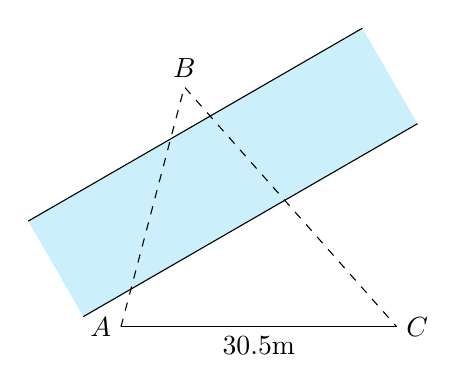
\begin{tikzpicture}[>=latex, scale=.7]
    \fill[rotate=30, cyan!20] (-.5,0.5) rectangle (6.5,2.5);
    \draw[rotate=30] (-.5,.5)--(6.5,.5)    ;
    \draw[rotate=30]  (-.5,2.5)--(6.5,2.5)    ;  
\draw[dashed] (0,0)node[left]{$A$}--(75.2:4.5)node[above]{$B$}--(5,0);
\draw (5,0)node[right]{$C$}--node[below]{30.5m}(0,0);


    \end{tikzpicture}
    \caption{第13题}
    \end{minipage}
    \begin{minipage}[t]{0.48\textwidth}
    \centering
    \begin{tikzpicture}[>=latex, scale=1.5]
    \draw (0,0)node[left]{$B$}--(3,-2)node[right]{$A$}--(1.5,-2.5)node[below]{$C$}--(0,0);
\draw[->] (0,0)--(0,.75)node[right]{北};
\draw[->] (1.5,-2.5)--(1.5,-2.5+.75);
\draw[->] (0,.5)  arc (90:-28:.5);
\node at (31:.5)[right] {$126^{\circ}$};
\draw[->] (0,.25)  arc (90:-56:.25);
\node at (17:.25)[right]{$148^{\circ}$};
\draw[->] (1.5,-2) arc (90:15:.5)node[above=10pt]{$78^{\circ}$};
    \end{tikzpicture}
    \caption{第15题}
    \end{minipage}
    \end{figure}

\item  某气象站每天定时施放气球进行高空观测,为了知道
气球离地面的高度,两观测员在$A,B$两点同时、同向
测得气球仰角$\alpha=45^{\circ}$, $\beta=34^{\circ}36'$, 且知道$A,B$两点相
距118米,求气球离地面的高度,已知测量仪器的高度为
1米(精确到1米)。
\item  在山顶铁塔上$B$处测得地面上一点的俯角$\alpha=54^{\circ}40'$,
在塔底$C$处测得点$A$的俯角$B=50^{\circ}1'$,已知铁塔$BC$部
分高27.3米,求山高$CD$(精确到1米)。

\begin{figure}[htp]
    \centering
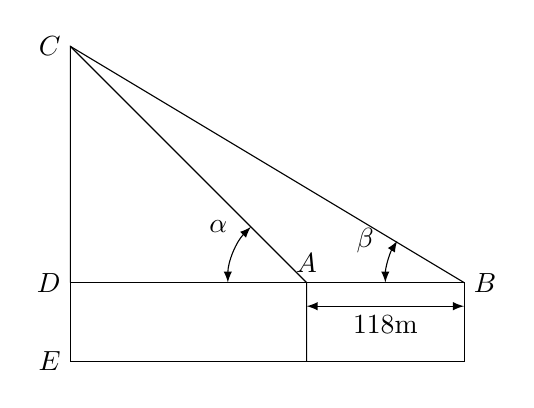
\begin{tikzpicture}[scale=1, >=latex]
\draw (0,0)node[left]{$E$} rectangle (5,1);
\draw (0,1)node[left]{$D$}--(0,4)node[left]{$C$}--(5,1)node[right]{$B$};
\draw (0,4)--(3,1)node[above]{$A$}--(3,0);

\draw[<->] (2,1) arc (180:90+45:1)node[left=5pt]{$\alpha$};
\draw[<->] (4,1) arc (180:180-32:1)node[left=5pt]{$\beta$};
\draw[<->] (5,.7) --node[below]{118m}(3,.7);
\end{tikzpicture}
    \caption{第16题}
\end{figure}

\end{enumerate}

\section*{复习题一}
\addcontentsline{toc}{section}{复习题一}
\begin{enumerate}
    \item 计算:
\begin{enumerate}
\item    $3^{0}+3^{-1}-\left(1\frac{7}{9}\right)^{0.5}$
\item   $\left[1-(0.5)^{-2}\right] \div\left(-\frac{27}{8}\right)^{\tfrac{1}{3}}$
\item    $\left(2 \frac{3}{5}\right)^{0}+4^{-2} \times\left(2 \frac{1}{4}\right)^{\tfrac{1}{2}}-(0.01)^{0.5}$
\item   $\left(2 \frac{10}{27}\right)^{-\tfrac{2}{3}}-\left[(0.01)^{\sin\tfrac{\pi}{6}}+\left(6 \frac{1}{4}\right)^{-0.5}\right]$
\end{enumerate}
\item 计算:
\begin{enumerate}
    \item $3^{\log_{3} 9}$
    \item $3^{1-\log _{3} 7}$
    \item $5^{2 \log _{5} 3}-15 \log _{5} 1+\log _{3} \frac{1}{9}$
    \item $4\lg 2+3 \lg 5-\frac{1}{5} \lg 5$
    \item $(\lg 5)^{2}+\lg 2 \cdot \lg 50$
    \item $\lg 5 \cdot \lg 20+(\lg 2)^{2}$
    \item $\lg 12.5-\lg  \frac{5}{8}+\lg\sin 30^{\circ}$
    \item $\log _{2} \cos \frac{\pi}{4}-\log _{2} \sin \frac{\pi}{6}$
    \item $\log _{3} \frac{1}{27}+\log _{\tfrac{1}{2}} 8+\log _{2} 8+\log _{4} 64$
    \item $\frac{5 \lg 6-\lg 3}{1+\frac{1}{2} \lg 0.36+\frac{1}{3} \lg 8}$
    \item $\left(\log _{9} 5\right) \cdot\left(\log _{25} 27\right)$
    \item $2^{\tfrac{1}{5 \log _{5}4}}$
\end{enumerate}

  \item 化简:
 \begin{enumerate}
    \begin{multicols}{2}
     \item $\frac{\left(a^{\tfrac{3}{5}}b^{-\tfrac{6}{5}}\right)^{-\tfrac{1}{2}}\sqrt[5]{a^4}}{\sqrt[5]{b^3}}$
     \item $\left(\frac{8x^{-3}}{\sqrt{y^3z^{-6}}}\right)^{-\tfrac{1}{3}}$
     \item $\sqrt[3]{\frac{8a^3b^6}{27c^3d^9}}$
     \item $8x^{-\tfrac{1}{3}}\sqrt{y^{-\tfrac{1}{3}}x\sqrt[4]{y^{\tfrac{4}{3}}}}$
     \item $\left(2x^{\tfrac{1}{2}}+3y^{-\tfrac{1}{4}}\right)\left(2x^{\tfrac{1}{2}}-3y^{-\tfrac{1}{4}}\right)$
     \item $\left(m^{\tfrac{3}{2}}+n^{\tfrac{3}{2}}\right)\div \left(m^{\tfrac{1}{2}}+n^{\tfrac{1}{2}}\right)$
     \item $\frac{a-b}{a^{\tfrac{1}{3}}-b^{\tfrac{1}{3}}}-\frac{a+b}{a^{\tfrac{1}{3}}+b^{\tfrac{1}{3}}}$
    \end{multicols}
     \item $(1-x^2)^{-\tfrac{1}{2}}-[(1+x)(1-x)]^{\tfrac{1}{2}}-x^2 [(1+x)(1-x)]^{-\tfrac{1}{2}}$
 \end{enumerate} 

 \item 利用对数进行计算:
 \begin{multicols}{2}
\begin{enumerate}
 \item $\frac{8.15^{2} \times \sqrt[3]{14.36}}{24.38 \times \sqrt{8.734}}$
 \item $\sqrt[5]{\frac{2.591^{4} \times \sqrt[3]{0.0836}}{1.147^{2}}}$
 \item $(-5.32)^{3}+\sqrt[4]{0.0294}$
 \item $\sqrt[3]{79.836+\sqrt{156.374}}$
\end{enumerate}
 \end{multicols}

\item \begin{enumerate}
    \item 已知 $\log _{12} 27=a$, 求证 $\log _{6} 16=\frac{4(3-a)}{3+a}$.
    \item 已知 $a^{2}+b^{2}=6 a b\; (a>0, b>0)$,
 求证 $\lg \frac{a-b}{2}=\frac{1}{2}(\lg a+\lg b)$.
\end{enumerate}

\item  解下面方程:
\begin{multicols}{2}
    \begin{enumerate}
        \item  $\begin{cases}
            5^{x}=2^{-y} \\ 
            5^{2+y}=2^{2-x}
        \end{cases}$
        \item  $\begin{cases}
            2^{x}=3^{y}\\ 
            2^{y-1}=3^{x-1}
        \end{cases}$
        \item $x^{\lg x+2}=1000$
        \item $\log_2\log_3\log_5x =0$
        \item $\begin{cases}
            x^5y^3=5\\x^2y^7=11
        \end{cases}$
\end{enumerate}
\end{multicols}

\item 下图表示曲柄机构装置的图样,连接杆$MK$的长$\ell=125$
cm, 曲柄$OK$的长$r=25$cm,连杆与汽缸的轴$OM$成$\alpha$角,
曲柄与同一轴成角$\phi$(例如$\phi=50^{\circ}$), 求活塞$M$的位移$x$
(这里$x$为活塞由左端位置所走的距离)。

\begin{figure}[htp]
    \centering
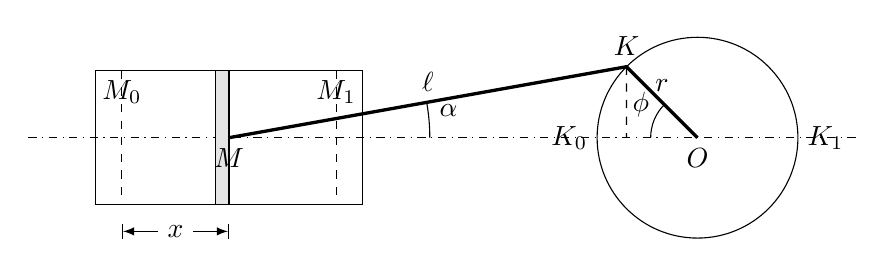
\begin{tikzpicture}[>=latex, scale=1.7]
    \draw[dashdotted] (-5,0)--(1.2,0);
    \draw (-4.5,.5) rectangle (-2.5,-.5);
    \draw (0,0) circle (.75);
    \node at (-.75,0)[left]{$K_0$};
    \node at (.75,0)[right]{$K_1$};
\draw [fill=gray!20](-3.5,.5) rectangle (-3.6,-.5);
\draw[very thick] (0,0)node[below]{$O$}--node[above]{$r$}(90+45:.75)node[above]{$K$}--node[above]{$\ell$}(-3.5,0)node[below]{$M$};
\draw [dashed](-4.3,.5)node[below]{$M_0$}--(-4.3,-.5);
\draw [dashed](-2.7,.5)node[below]{$M_1$}--(-2.7,-.5);
\draw (-.35,0) arc (180:180-45:.35)node[left=2pt]{$\phi$};
\draw[dashed] (90+45:.75)--(-.75/1.414,0);
\draw[|<->|] (-4.3,-.7)--node[fill=white]{$x$}(-3.5,-.7);

\draw (-2,0) arc (0:10:1.5);
\node at (-2,.2)[right]{$\alpha$};
\end{tikzpicture}
    \caption{第7题}
\end{figure}

\item 如图,两个建筑物水平距离为32.6米,从$A$点观测$B$点
的俯角是$35^{\circ}12'$, 观测$C$点的俯角为$43^{\circ}24'$, 求此二建
筑物的高。

\begin{figure}[htp]
    \centering
\begin{tikzpicture}[>=latex]
\fill [pattern=north east lines] (0,0) rectangle (-.5,4);   
\draw (0,0)--(0,4)node[above]{$A$}--(3,4);
\fill [pattern=north east lines] (5,0) rectangle (5.5,1);   
\draw (5,0)--(5,1)--(5.5,1);
\draw (0,0)--(0,-1);
\draw (5,0)--(5,-1);
\draw[<->](0,-.5)--node[fill=white]{32.6m}(5,-.5);
\node at (0,-.2) [left]{$D$};
\node at (5,-.2) [right]{$C$};
\draw (0,4)--(5,0);\draw (0,4)--(5,1)node[above]{$B$};
\draw(-1,0)--(6,0);

\end{tikzpicture}
    \caption{第8题}
\end{figure}

\item 一只渔船在航行中不幸遇险,发出警报,在遇险南西10
海里处有一具货轮,收到警报后立即侦察,发现这只渔
船的航向是东$15^{\circ}$南,正在用每小时9海里的速度向某
小岛靠近,如果要在40分钟内把这只渔船营救出来,求
货轮航行方向和速度(精确到分)。
\item 
在塔的正西处$A$点测得塔顶的仰角是$45^{\circ}$, 在它的东南
处$B$点测得仰角是$60^{\circ}$, $AB$相距为266尺。求塔高。











\end{enumerate}


